\PassOptionsToPackage{table}{xcolor}
\documentclass[sigchi]{acmart}
% \documentclass{sigchi}
% \settopmatter{printacmref=false} % Removes citation information below abstract
% \renewcommand\footnotetextcopyrightpermission[1]{} % removes footnote with conference information in first column
% Load basic packages
\usepackage{booktabs} % For formal tables
\usepackage{balance}  % to better equalize the last page
\usepackage{graphics} % for EPS, load graphicx instead
\usepackage[T1]{fontenc}
\usepackage{booktabs}
\usepackage{textcomp}
\usepackage{xspace}
\usepackage{setspace}
\usepackage[textsize=tiny]{todonotes}
% Some optional stuff you might like/need.
\usepackage{microtype} % Improved Tracking and Kerning
% \usepackage[all]{hypcap}  % Fixes bug in hyperref caption linking
\usepackage{ccicons}  % Cite your images correctly!
% \usepackage[utf8]{inputenc} % for a UTF8 editor only
\usepackage{verbatim}
\usepackage{relsize}
\usepackage{etoolbox}
\usepackage{lipsum}   % for filler text
\usepackage{setspace} % for \onehalfspacing and \singlespacing macros
\usepackage[normalem]{ulem}
\usepackage{fixltx2e}
\usepackage{amsmath}
\usepackage{amssymb}
\usepackage{afterpage}
\usepackage[htt]{hyphenat}
\usepackage{microtype}                 % use micro-typography (slightly more compact, better to read)
\PassOptionsToPackage{warn}{textcomp}  % to address font issues with \textrightarrow
\usepackage{times}                     % we use Times as the main font
\renewcommand*\ttdefault{txtt}         % a nicer typewriter font
\usepackage{tabu}                      % only used for the table example
\usepackage{booktabs}                  % only used for the table example
% \usepackage[linesnumbered,ruled]{algorithm2e}
\usepackage{algorithm}
\usepackage[noend]{algpseudocode}
\usepackage[export]{adjustbox}
\usepackage{tikz}
\usetikzlibrary{shapes,arrows}
\usepackage{subfig}
\raggedbottom
\DeclareMathOperator*{\argmax}{arg\,max}
% llt: Define a global style for URLs, rather that the default one
\makeatletter %making the spacing between paragraphs less dramatic
\def\url@leostyle{%
  \@ifundefined{selectfont}{
    \def\UrlFont{\sf}
  }{
    \def\UrlFont{\small\bf\ttfamily}
  }}
\makeatother

\newenvironment{denselist}{
    \begin{list}{\small{$\bullet$}}%
    {\setlength{\itemsep}{0ex} \setlength{\topsep}{0ex}
    \setlength{\parsep}{0pt} \setlength{\itemindent}{0pt}
    \setlength{\leftmargin}{1.5em}
    \setlength{\partopsep}{0pt}}}%
    {\end{list}}

\newcommand{\squishlist}{
   \begin{list}{$\bullet$}
    { \setlength{\itemsep}{0pt}
      \setlength{\parsep}{2pt}
      \setlength{\topsep}{0pt}
      \setlength{\partopsep}{0pt}
      \leftmargin=25pt
\rightmargin=0pt
\labelsep=5pt
\labelwidth=10pt
\itemindent=0pt
\listparindent=0pt
\itemsep=\parsep
    }
}
\newcommand{\origcolor}[1]{\color[HTML]{7C0FFF}{#1}}
\newcommand{\diffcolor}[1]{\color[HTML]{FA7300}{#1}}
\newcommand{\squishend}{\end{list}}
\newcommand{\npar}{\par \noindent}
% use extensively to toggle between paper and TR
\newcommand{\eat}[1]{}
\newcommand{\papertext}[1]{#1}
% \newcommand{\tr}[1]{{\leavevmode\color{lightgray}{#1}}}
\newcommand{\tr}[1]{}
\newcommand{\boldpara}[1]{\textbf{\paragraph{#1}}}
% de-facto paragraph format
\newcommand{\stitle}[1]{\par\noindent\textbf{#1}}
\newcommand{\opt}[1]{{\leavevmode\color{purple}{#1}}} %optional if need cut (may go into TR)
\newcommand{\ccut}[1]{} %confirmed cut
\newcommand{\system}{\textsc{VisPilot}\xspace}
\newcommand{\shortsystem}{\textsc{VP}\xspace} %shorthand for system
\newcommand{\cluster}{\textsc{Cluster}\xspace}
\newcommand{\BFS}{\textsc{BFS}\xspace}
\newcommand{\fem}{\texttt{Female}\xspace}
\newcommand{\blk}{\texttt{African-American}\xspace}
\newcommand{\blkfem}{\texttt{African-American Female}\xspace}

\newcommand{\agp}[1]{\textcolor{blue}{Aditya: #1}}
\newcommand{\dor}[1]{\textcolor{green}{Doris: #1}}
\newcommand{\hdev}[1]{\textcolor{magenta}{Himel: #1}}
\newcommand{\haz}[1]{\textcolor{orange}{Hazem: #1}}
\newcommand{\change}[1]{{\leavevmode\color{red}#1}}
\newcommand{\achange}[1]{{\leavevmode\color{blue}#1}}

\urlstyle{leo}
% \AtBeginEnvironment{quote}{\small}
\renewenvironment{quote}{%
  \vspace{-3pt}
   \list{}{%
     \leftmargin0.15cm
     \rightmargin\leftmargin
   }
   \item\relax
}
{\vspace{-3pt} \endlist}

% To make various LaTeX processors do the right thing with page size.
\def\pprw{8.5in}
\def\pprh{11in}
\special{papersize=\pprw,\pprh}
\setlength{\paperwidth}{\pprw}
\setlength{\paperheight}{\pprh}
\setlength{\pdfpagewidth}{\pprw}
\setlength{\pdfpageheight}{\pprh}

\newcommand*\OK{\ding{51}}
\renewenvironment{quote}{%
   \list{}{%
     \leftmargin0.15cm
     \rightmargin\leftmargin
   }
   \item\relax
}
{\endlist}
\copyrightyear{2019}
\acmYear{2019}
% \setcopyright{acmlicensed}
\setcopyright{acmcopyright}
\acmBooktitle{IUI Conference on Intelligent User Interfaces Proceedings (IUI 2019), March 17--20, 2019, Los Angeles, USA}
\acmPrice{15.00}
\acmISBN{978-1-4503-5970-2/19/05}
\acmDOI{10.1145/XXXXXX.XXXXXX}
% Authors, replace the red X's with your assigned DOI string during the rightsreview eform process.

\settopmatter{printacmref=true}
\fancyhead{}

%%%%%%%%%%%%%%%%%%%%%%%%%%%%%%%%%%%%%%%%%%%%%%%%%%%%%%%%%%%%%%%%
%%%%%%%%%%%%%%%%%%%%%% START OF THE PAPER %%%%%%%%%%%%%%%%%%%%%%
%%%%%%%%%%%%%%%%%%%%%%%%%%%%%%%%%%%%%%%%%%%%%%%%%%%%%%%%%%%%%%%%%

\begin{document}
\author{Doris Jung-Lin Lee$^\dagger$, Himel Dev$^\dagger$, Huizi Hu$^\dagger$, Hazem Elmeleegy$^\star$, Aditya Parameswaran$^\dagger$}
\affiliation{
  \institution{$^\dagger$University of Illinois, Urbana-Champaign, $^\star$Google, Inc.}
}
\email{jlee782|hdev3|huizihu2|adityagp@illinois.edu, elmeleegy@google.com}


% \author{Doris Jung-Lin Lee}
% \affiliation{
%   \institution{University of Illinois, Urbana-Champaign}
% }
% \email{jlee782@illinois.edu}

% \author{Himel Dev}
% \affiliation{
%   \institution{University of Illinois, Urbana-Champaign}
% }
% \email{hdev3@illinois.edu}
% \author{Huizi Hu}
% \affiliation{
%   \institution{University of Illinois, Urbana-Champaign}
% }
% \email{huizihu2@illinois.edu}
% \author{Hazem Elmeleegy}
% \affiliation{%
%   \institution{Google, Inc.}
% }
% \email{elmeleegy@google.com}

% \author{Aditya Parameswaran}
% \affiliation{%
%   \institution{University of Illinois, Urbana-Champaign}
% }
% \email{adityagp@illinois.edu}
%\title{Avoiding the Drill-down Fallacy with Storyboard: Assisted and Accelerated Data Exploration Through Data Subsets}
\title{Avoiding Drill-down Fallacies with {\em VisPilot}: Assisted Exploration of Data Subsets}
\begin{abstract}
As datasets continue to grow in size and complexity,
exploring multi-dimensional datasets remain challenging for analysts.
A common operation during this exploration is drill-down---understanding
the behavior of data subsets by \change{progressively} adding filters.
While widely used, in the absence of careful attention towards confounding factors,
drill-downs could lead to inductive fallacies.
Specifically, an analyst may end up being \lq\lq deceived\rq\rq\ into thinking that a deviation in trend is attributable to a local change, when in fact \change{it is a more general phenomenon};
we term this the \change{{\em drill-down fallacy}}.
\change{One way to avoid falling prey to drill-down fallacies}
is to exhaustively explore all potential drill-down paths,
which quickly becomes infeasible \change{on complex datasets with many attributes}.
We present \system, an accelerated visual data exploration tool that guides analysts
\change{through the} key insights in a dataset, while avoiding drill-down fallacies.
Our user study results show that \system helps analysts discover
interesting visualizations, understand attribute importance,
and predict unseen visualizations better than other summarization baselines.
%towards meaningful insights for a variety of tasks.
\end{abstract}
\maketitle
 \author{Doris Jung-Lin Lee, Himel Dev, Huizi Hu, Hazem Elmeleegy, Aditya Parameswaran}


\keywords{exploratory data analysis, visualization recommendation.}
% \begin{teaserfigure}
%   \centering
%   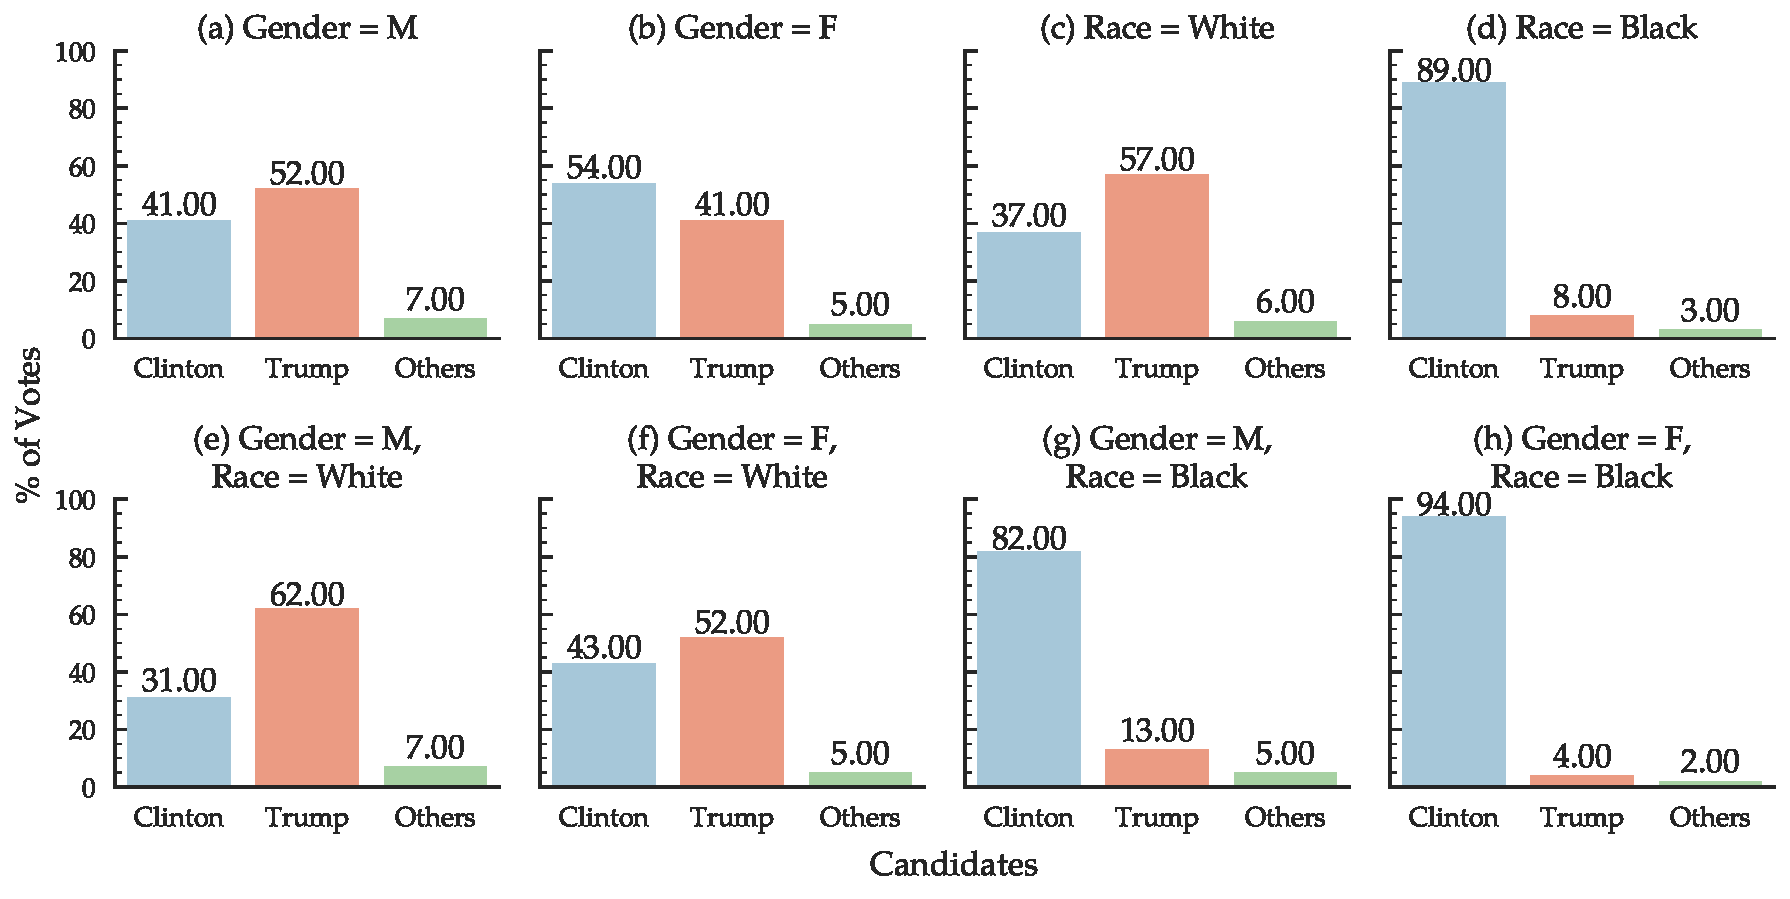
\includegraphics[width=\linewidth]{figures/US_Election_Example.pdf}
%   \caption{A set of visualizations from the 2016 Election polls. These visualizations show the percentage of votes for three candidates (Donald Trump, Hilary Clinton, and Others) in different demographic groups (based on race and gender).}
%   \label{fig:elections_example}
% \end{teaserfigure}

%The task of navigating through a large, multidimensional dataset is a common challenge in exploratory analysis. Due to limitations on the number of visualizations that an analyst can examine at one time, the narrow scope of drill-downs can often lead to inductive fallacies. %Not only is manual drill-down and roll-up on data subsets tedious and inefficient for the analyst, the massive space of data subsets, lack of interesting patterns in most data subsets, fallacies of spurious correlations, and pitfalls of statistical paradoxes calls for a systematic and effective way for analysts to make sense of and navigate through the large space of possible visualizations.
%In this paper, we present \system, an interactive visualization recommendation system provide safe guarantee during drill-down exploration by picking the proper visualization reference that leads to interesting and informative trends. Given a dataset and the x and y axes of interest, \system\ intelligently explores the lattice of equivalent visualizations across data subsets, and recommends interesting and informative visualizations. The recommended visualizations are then displayed in an interactive dashboard, where the visualizations are organized into a hierarchical layout. Our evaluation study shows that visualization dashboards generated by \system\ are interpretable and leads to higher performance in data analytic tasks compared to the competing baselines.

% \begin{figure*}[bht]
% \centering
% 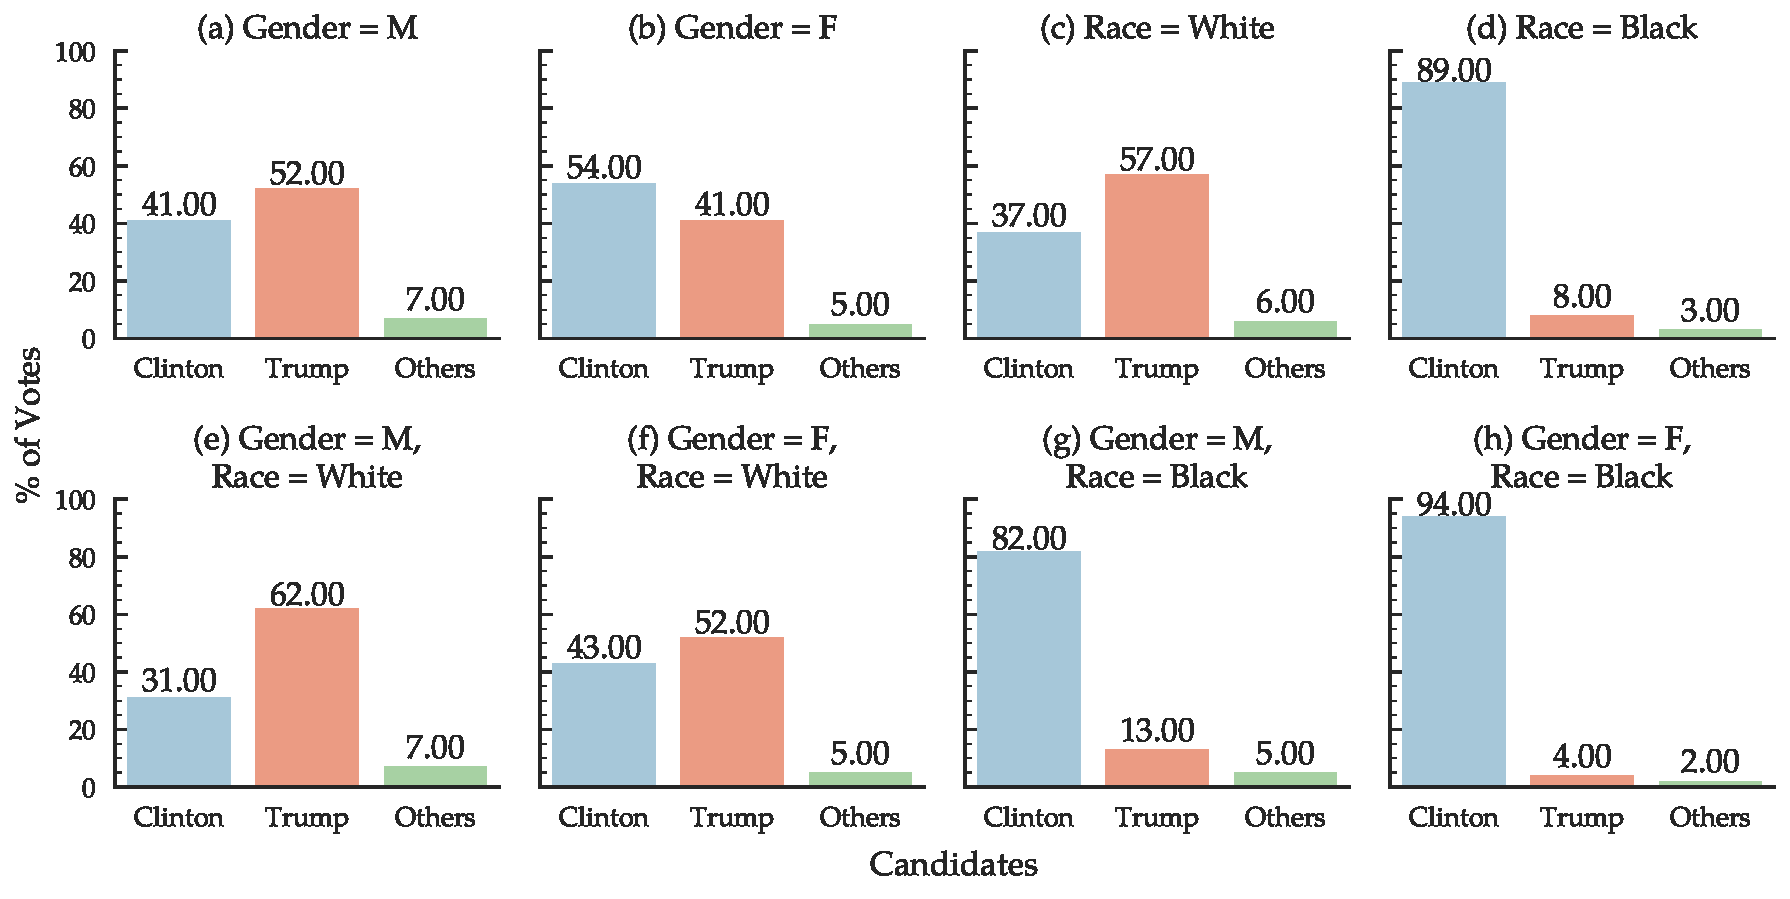
\includegraphics[width=\linewidth]{figures/US_Election_Example.pdf}
% \caption{A set of visualizations from the 2016 Election polls. These visualizations show the percentage of votes for three candidates (Donald Trump, Hilary Clinton, and Others) in different demographic groups (based on race and gender).}
% \label{fig:elections_example}
% \end{figure*}

\section{Introduction}

%\hdev{Let's take a step back, and look at the current flow in introduction. In the first paragraph, we vaguely motivate what can be considered as collective insights. In second paragraph, we try to connect the idea of collective insights with the challenges of data subset exploration. In third paragraph, we introduce two concepts: visual summarization, and distribution awareness. We do not clearly state what these two means. There's an example that conveys what could be captured through pattern or trend mining. In the fourth paragraph, we present an example to convey some specific challenges of visual summarization. The fifth paragraph states our contributions. My suggestion is to immediately jump into business by saying what we mean by distribution awareness, why is it important, and why is this challenging. We have the contents lying around already, it's just a matter of clearly stating these three aspects, preferably without using new abstractions.}

Common analytics tasks, such as causal inference, feature selection, and outlier detection requires studying the distributions or patterns at different granularities of data [Refs]. For example, a campaign manager may study the voting patterns in different demographics (based on race, gender, social class etc.) using the 2016 US election exit polls\footnote{\url{https://edition.cnn.com/election/2016/results/exit-polls}} to identify the nonconformist demographic groups. Visual analysis is the \emph{de facto} approach for performing such analytics tasks [Refs], where an analyst constructs visualizations to capture the distributions at different subsets of data. The goal of this visual analysis is to extract meaningful insights---when a set of visualizations along with human interpretation leads to informative and interesting facts arising from the distributions.

However, without knowing \textit{what} subset of data contains an interesting distribution, manually exploring all possible data subsets can be tedious and inefficient for an analyst. For example, the aforementioned campaign manager could construct bar charts for different demographics, where x-axis shows the election candidates and y-axis the percentage of votes for these candidates. Subsequently, he could compare these bar charts to understand how voting pattern changes across different demographics. Both of these exercises, first, constructing the large number of visualizations corresponding to all possible data subsets, and then, navigating through this large space of visualizations to draw meaningful insights is challenging. Currently, there is no systematic way to perform these exercises. 

To this end, we present \system, an interactive visualization summarization system that automatically selects a small set of visualizations to summarize the data distributions within a dataset in an informative manner. When analysts inspect informative visualizations that cover these insights, they associate particular sets of attributes to typical trends and observed patterns. We define this aspect of dataset understanding as \emph{distribution awareness}. For example, we observe that in Figure~\ref{fig:elections_example}, most of the visualizations has `Clinton' and `Trump' as comparably-sized bars with `Others' being a small fraction of the overall (a,b,c,e,f), whereas visualizations involving the Black population is highly skewed towards `Clinton' (d,g,h). Since human analysts have limited memory and attention, it is often impossible to visualize all possible data subsets. An ideal summarization system should display visualizations that enables users to gain maximal distribution awareness of the typical trends within a dataset. 

%Even after constructing the visualizations for all possible data subsets, which itself is a daunting task, currently there is no systematic way for our campaign manager to make sense of or even navigate through this large space of possible visualizations to draw meaningful insights. 

%\par The goal of visual analysis is to extract meaningful stories or insights from the data. Individual visualizations represent simple ``factoids'' portraying one aspect of the data. Meaningful insights arise when a group of factoids work in conjunction, along with human interpretation, to produce informative and interesting facts. 
%\par However, without knowing \textit{what} subset of the data would be interesting to visualize, manual drill-downs and roll-ups on all possible filter combinations can be tedious and inefficient for analysts. In many data analytics scenarios, analysts have an x and y axis of interest and want to explore data subsets corresponding to different filtering criteria. For example, a campaign manager may be interested in looking at bar chart visualizations of x as the voted candidate and y as the percentage of votes for the 2016 US elections exit polls with different filter combinations on demographics information, such as gender, income, race, states, and responses to different survey questions\footnote{\url{https://edition.cnn.com/election/2016/results/exit-polls}}. The analyst would have to compare across a combinatorially large space of different data subsets by iteratively changing the filter criterion of a visualization to understand how the relationship between the x and y variables change across data subsets. Even if the analyst had plotted visualizations for all possible data subsets, currently there is no systematic and effective way for an analyst to make sense of and navigate through the large space of possible visualizations to draw meaningful insights. 
%\par To this end, we present \system, an interactive visualization summarization system that automatically selects a small set of visualizations to summarize the data distributions within a dataset in an informative manner. When analysts inspect informative visualizations that cover these insights, they associate particular sets of attributes to typical trends and observed patterns. We define this aspect of dataset understanding as \emph{distribution awareness}. For example, we observe that in Figure~\ref{fig:elections_example}, most of the visualizations has `Clinton' and `Trump' as comparably-sized bars with `Others' being a small fraction of the overall (a,b,c,e,f), whereas visualizations involving the Black population is highly skewed towards `Clinton' (d,g,h). Since human analysts have limited memory and attention, it is often impossible to visualize all possible data subsets. An ideal summarization system should display visualizations that enables users to gain maximal distribution awareness of the typical trends within a dataset. 
%\par However, finding effective visualizations to summarize a dataset is not as trivial as picking individual visualizations that maximizes some statistical measure, such as deviation~\cite{Vartak2015}, coverage~\cite{Sarvghad2017}, or significance testing~\cite{Anand2015}, which can often result in misleading summarizations. Consider an elections campaign manager who is allocating the advertisement budget to be spent on different demographic populations to target for an upcoming election by investigating the voting patterns across different demographic groups. He performs a randomized permutation testing between the gender and race attributes and finds that the voting pattern of black females is drastically different from the voting pattern of general female population and allocates the his advertisement funds to target the black female population. \dor{Himel, can you check if this example makes sense? or should we say chi2? chi2 just give you columnar correlation info not at the attribute-level info? although probably only a deviation based comparison can give you a comparison like this.} While black females do defy the trends of general females, the comparison is incomplete, since it ignores the fact that black females follows very closely to the distribution of the voting behavior of the black population, so the proper subpopulation to target should be the black population rather than the more specific black female population.
%\par The above example showcases a scenario where the selection of an improper reference (female) for comparing the visualization (black female) against results in misleading insights. In \system, we formulate an objective where a visualization is \emph{actually} interesting when it deviates from and can not be explained by \emph{even} its most informative reference. \dor{can we add an example here?} Our user study results described in Section~\ref{sec:userstudy} shows that this notion of informative interestingness can guide an analyst towards more meaningful stories for further investigation. 
\par The contribution of this paper include: 
\begin{denselist}
\item Proposing the novel problem of visualization summarization and use cases highlighting the importance of \textit{distribution awareness} in dataset understanding (Section~\ref{sec:distributionaware}), %inform  visualization understanding and analytical tool designs
\item Formulating the structure and utility of the visualization search space (\emph{lattice}) using a user expectation model motivated by our formative study (Section~\ref{sec:datamodel}),
\item Designing efficient algorithms and optimizations to identify a set of informatively connected interesting visualizations (Section~\ref{sec:system}),  
\item Presenting an interactive visualization dashboard interface that adopts a simple and intuitive hierarchical lattice layout (Section~\ref{sec:interaction}),
\item Demonstrate the efficacy of our system through a user study evaluation (Section~\ref{sec:userstudy}).
\end{denselist}
%!TEX root = main.tex
% \section{Towards Informative Exploration}
\change{\section{Problem Formulation\label{sec:problem}}}
In this section, we first describe how analysts
manually explore the space of data subsets.
We then introduce \change{three design principles
for a system that can automatically guide analysts to the key insights}.
% \subsection{Manual Exploration via Drill-Downs}

\change{\subsection{Manual Exploration: Approach and Challenges}}
During visual data exploration,
an analyst may need to explore different subsets
of the data \change{that together form a combinatorial \emph{lattice}}.
Figure~\ref{fig:elections_example}
shows a partial lattice for the 2016 US election dataset.
The lattice contains the overall visualization
with no filter at the first level,
all visualizations with a single filter
at the second level \change{(such as \fem)},
all visualizations with two filters at third level,
and so on.
Analysts explore such a combinatorial lattice
from top to bottom, by generating and examining
visualizations with increasing levels of specificity.
In particular, analysts perform \emph{drill-downs}~\cite{Gray1997}
to access data subsets at lower levels by
adding one filter at a time
\change{(such as adding \blk to \fem along the purple path)}
and visualize
\change{their measures of interest for each data subset---in
this case the percentage of votes for each candidate}.
Further, as analysts perform drill-downs,
they use the most recent visualization
in the drill-down path---the {\em parent}---as a \change{{\em reference}}
to establish what they expect to see in the
\change{next visualization in the path---the {\em child}}.
In Figure~\ref{fig:elections_example},
the visualizations \fem and \blk
are the \emph{parents} of the \blkfem visualization,
explored along the purple and orange path respectively.

\par \change{As we saw in the purple path
in Figure~\ref{fig:elections_example},
while performing drill-downs,
analysts may detect a local deviation
(we will formalize these and other notions subsequently)
between
a parent and a child to be significant.
For example, they may be surprised by the fact
that the \fem and \blkfem
visualizations are very different from each other,
and may
find this to be a novel insight.
However, this deviation is a result of \fem
not being an
{\em informative}
parent or reference for \blkfem---instead, it is a
{\em deceptive} reference.
Here, a different parent, \blk,
is the most informative parent or reference of \blkfem
because it is the parent that exhibits the
least deviation relative
to \blkfem.
Here, the \blkfem visualization
is not really all that surprising given the \blk
visualization.
We refer to this phenomenon of being deceived by
a local difference or deviation relative to a deceptive
reference as an instance of the {\em drill-down fallacy}.
One way to avoid such fallacies is to ensure that one or more
informative parents
are present for each visualization so that analysts
can contextualize the visualization accurately.
While this fallacy is applicable to any
chart type that can be described as a
probability distribution over data
(e.g., pie charts, heatmaps),
we will limit our discussion to bar charts for brevity.}

% \subsection{Three Elements of Informative Exploration}
\change{\subsection{The ``3S'' Design Principles}}
Our goal is to help analysts discover
the key insights in a dataset while avoiding drill-down fallacies.
We \change{outline}
three essential principles for
finding such insights---the three S's:
\emph{safety}, \emph{saliency}, and \change{\emph{succinctness},
and progressively layer these principles to formalize
a measure of utility for a network of visualizations}.
We adopt these principles to
develop a visual exploration tool
that \change{automatically generates
a network of visualizations conveying the key
insights in a multidimensional dataset}.

\subsubsection{Safety}
\change{To prevent
drill-down fallacies,
we ensure {\em safety}---by making sure
that informative parents are present
to accurately contextualize visualizations.
A parent is said to be {\em informative}
if its data distribution closely follows the child
visualization's data distribution,
since the presence of the parent allows
the analyst to form an accurate mental model
of what to expect from the child visualization.
We compute the informativeness of
the $j^{th}$ parent $V_i^j$
for a visualization $V_i$
as the similarity between their data distributions
measured using a distance function $D$.
For bar charts, the data distribution refers to
the height of bars assigned to the categories labeled by the x-axis,
suitably normalized.
Accordingly, the computed distance
$D(V_i, V_i^j)$
refers to the sum of the distances
between the normalized heights of bars across different categories.
Quantifying deviation using distances between normalized versions of visualizations
in this manner is not a novel idea---we leverage prior work for this~\cite{Vartak2015,Siddiqui2017,Macke2018,Ding2016}.
The specific distance measure $D$ is not important; while we use the Euclidean metric,
we can easily work with other common distance metrics such as Kullback-Leibler Divergence and Earth Mover's distance~\cite{Vartak2015}.
The most informative parent $V_i^\dagger$ for a visualization $V_i$ is
the one whose data distribution is most similar to $V_i$.
}
%The distance $D(V_i, V_i^j)$ is computed based on the probability distributions represented by each visualization (in this case, a vector of bar values). \tr{For example, based on the Figure~\ref{fig:elections_example} example, the Euclidean distance between \fem ($V_i^j$=[54,41,5]) and \blkfem ($V_i$=[94,4,2]) is 54.57.} sqrt((94-54)**2+(41-4)**2+3**2)

\begin{equation}
    V_i^\dagger= \underset{V_i^j}{argmin}\ D(V_i, V_i^j)
\end{equation}
\change{Instead of insisting that the most informative
parent is always present to contextualize a given child visualization,
we relax our requirement somewhat: we don't need {\em the
most} informative parent to be present, just {\em an} informative parent.
We define a parent to be informative (denoted $V_i^*$) if its distance from the child falls within a threshold $\theta\%$ of the
most informative parent---the default is set to 90\%
and adjustable by the user.}
\cut{
    We regard a parent visualization as informative if its distance from the child visualization falls within a threshold $\theta\%$ compared to the most informative parent:
    \begin{equation}
        V_i^{*, \theta} = \{V_i^j : \frac{D(V_i, V_i^*)}{D(V_i, V_i^j)} \geq \theta\}
    \end{equation}
    For example in Figure~\ref{fig:elections_example}, while both \blk and \fem visualizations are considered parents of the \blkfem visualization, only the \blk visualization is considered an informative parent of the \blkfem population, for any values of $\theta \geq 11\%$ via the Euclidean distance metric.
}
\subsubsection{Saliency}
\change{Simply ensuring that
informative parents are present is insufficient;
we also want to emphasize {\em saliency} by
identifying visualizations that convey new information.
In general, a visualization is deemed to be \emph{interesting}
if its underlying data distribution differs
from that of its parents,
and thus offers new unexpected information or insight.
Such distance-based notions of interestingness
have been explored in past work~\cite{Correll2016,Itti2009,Vartak2015},
where a large distance from some reference visualization
indicates that the selected visualization is interesting.
We deviate from this prior work in two ways:
first, we concentrate on {\em informative} interestingness,
where the interestingness of a child visualization
is only defined with respect to informative parent references.
Second, we weigh the interestingness by the proportion of the
population captured by the child visualization.
(That is, when a deviation is manifested in a larger population,
it is deemed to be more significant and therefore more interesting.)
Thus, we define the utility of a visualization $V_i$, $U(V_i)$ as follows:
 $$
    U(V_i)=
\begin{cases}
     \frac{|V_i|}{|V_i^*|} \cdot D(V_i, V_i^*) & \text{if } V_i^* \text{ is present}\\
    -\infty             & \text{otherwise}
\end{cases}
$$
That is, the utility or interestingness of a visualization
is the distance between the visualization and its informative
parent, if present\footnote{If multiple informative parents, $V_i^*$, are present for a given visualization, $V_i$, then $U(V_i)$ is defined in terms of the most informative parent present.}. To incorporate the effect of subpopulation size into our objective function, we multiply the distance $D(V_i, V_i^*)$ between an informative parent $V_i^*$ and a child visualization $V_i$ by the ratio of their sizes.
Notice that the objective $U$ has a minimax form~\cite{wiki:minimax},
in that informativeness aims to minimize the distance between parent and child,
while interestingness aims to maximize the resulting minimum distance.
For convenience, we define $U(V_0)$, where $V_0$ is the overall visualization,
to be $1$, which is the maximum value that the expression $\frac{|V_i|}{|V_i^*|} \cdot D(V_i, V_i^*)$ can take, ensuring that the overall visualization
is always valuable to include.
}

\subsubsection{Succinctness}
\change{
We cannot possibly display all of the visualizations
in the lattice of data subsets: this lattice scales
exponentially in the number of attributes.
Instead, we aim for {\em succinctness},
where we only select a subset $S$ of size $|S| = k$ from all the visualizations.
We define the utility of $S$ as follows:
$$U(S) = \sum_{V_i \in S}{U(V_i)}$$
In this subset, for every visualization except for the overall
visualization, one of its informative
parents must be present (otherwise $U = -\infty$).
Thus, this subset ends up being a connected network
(a sub-graph of the overall lattice) rooted at the overall visualization,
ensuring that for each visualization, there is an informative parent available
for context.
We can now formally define our problem statement.
\par \textsc{Problem.} \textit{Given a dataset and user-provided X, Y attributes,
select a subset $S$ of $|S| = k$ visualizations from the lattice of data
subsets $\mathcal{L}$, such that $U(S)$ is maximized.}
\\
Thanks to how we have defined $U$, $S$ will include the overall visualization,
corresponding to the entire dataset with no filter. And,
for each visualization in $S$ except the overall one,
at least one of its informative parents will be present in $S$.
This network of visualizations $S$ can be displayed on a dashboard.
}
% To succinctly convey insights, we concentrate on \emph{summarization}---identifying a group of visualizations that collectively contain informative insights. Since our aim is to identify a unified narrative, instead of discrete insights, we enforce that any selected visualization must have at least one of its informative parents present in the dashboard. Specifically, we identify a set of $k$ connected visualizations that collectively maximize the sum of the proposed utility $U(V_i)$ across each selected visualization, $V_i$, and thus succinctly convey informative insights, more formally stated as follows:
% \par \textsc{Problem.} \textit{Given a dataset and user-provided X, Y attributes, select $k$ visualizations from the lattice of data subsets $\mathcal{L}$ to be included in the dashboard, such that:
% \\ (i) one of the selected visualization is the overall visualization, corresponding to the entire dataset with no filter;
% \\ (ii) for each visualization except for the overall, at least one of its informative parents is present in the $k$ visualizations;
% \\ (iii) the $k$ selected visualizations maximize the total utility $\sum_{V_i \in \mathcal{L}} U(V_i)$ as defined above.
% }
% and aggregation function G, a lattice $\mathcal{L}$ consisting of visualizations $V_i$ for all possible filter $F_i$ that could be constructed from dataset D:}
% \\ \texttt{$V_i$ = SELECT X, G(Y) FROM D WHERE $F_i$ GROUP BY X}
% \\ \textit{find k visualizations from $\mathcal{L}$ to include in dashboard $\mathcal{S}$, such that the total utility $\sum_{V_i \in \mathcal{L}} U(V_i)$ as defined above is maximized, while enforcing that all $V_i \in \mathcal{S}$ is connected.}
\change{Since the edges between non-informative parents to children are not pertinent to the solution, we can remove those edges from the lattice, leaving only the edges from the informative parents to the children. Then, we are left with an arbitrary graph, from which we need to select a rooted subgraph of size $k$, with greatest utility $U$.}
\par \tr{For arbitrary distance metrics $D$, we can show that our problem is {\sc NP-Hard} via a reduction from the AND-graph prerequisite problem, which has been shown to be {\sc NP-Hard} in ~\cite{Parameswaran2010}. Similar to our problem, in the AND-graph prerequisite problem, all prerequisites need to be taken before a node can be selected. Both the scoring function in the prerequisite problem and the distance-based utility in our problem are non-negative and independent of selection order. Furthermore, both the AND-graph in the prerequisite problem and our lattice have only directed edges across neighboring levels (i.e. only edge connections from n$\rightarrow$n+1). Based on our informativeness criteria, some directed edges may not be present in the graph. These pruned edges are equivalent to the AND-graph case where the score is zero. For a distance metric D, two nodes are discernable if the distance between them is zero. Hence, we prove by bijection that the two problems are equivalent and thereby proving that our problem is NP-hard.}
% Unfortunately, the problem of finding a
% connected subgraph in a lattice with
% maximum total edge utility is known
% as the \emph{maximum-weight connected subgraph problem}~\cite{ErnstAlthaus2009}
% and is known to be {\sc NP-Complete}~\cite{Parameswaran2010}.
% \agp{This doesn't actually show that our problem is hard. We need to reduce max-weighted subgraph to our problem, not the other way around. I am leaving a pointer here to think about it later.}
\change{Next, we design an approximate algorithm
 to solve this problem.}

%!TEX root = main.tex
\begin{figure}[h!]
\centering
\vspace{-10pt}
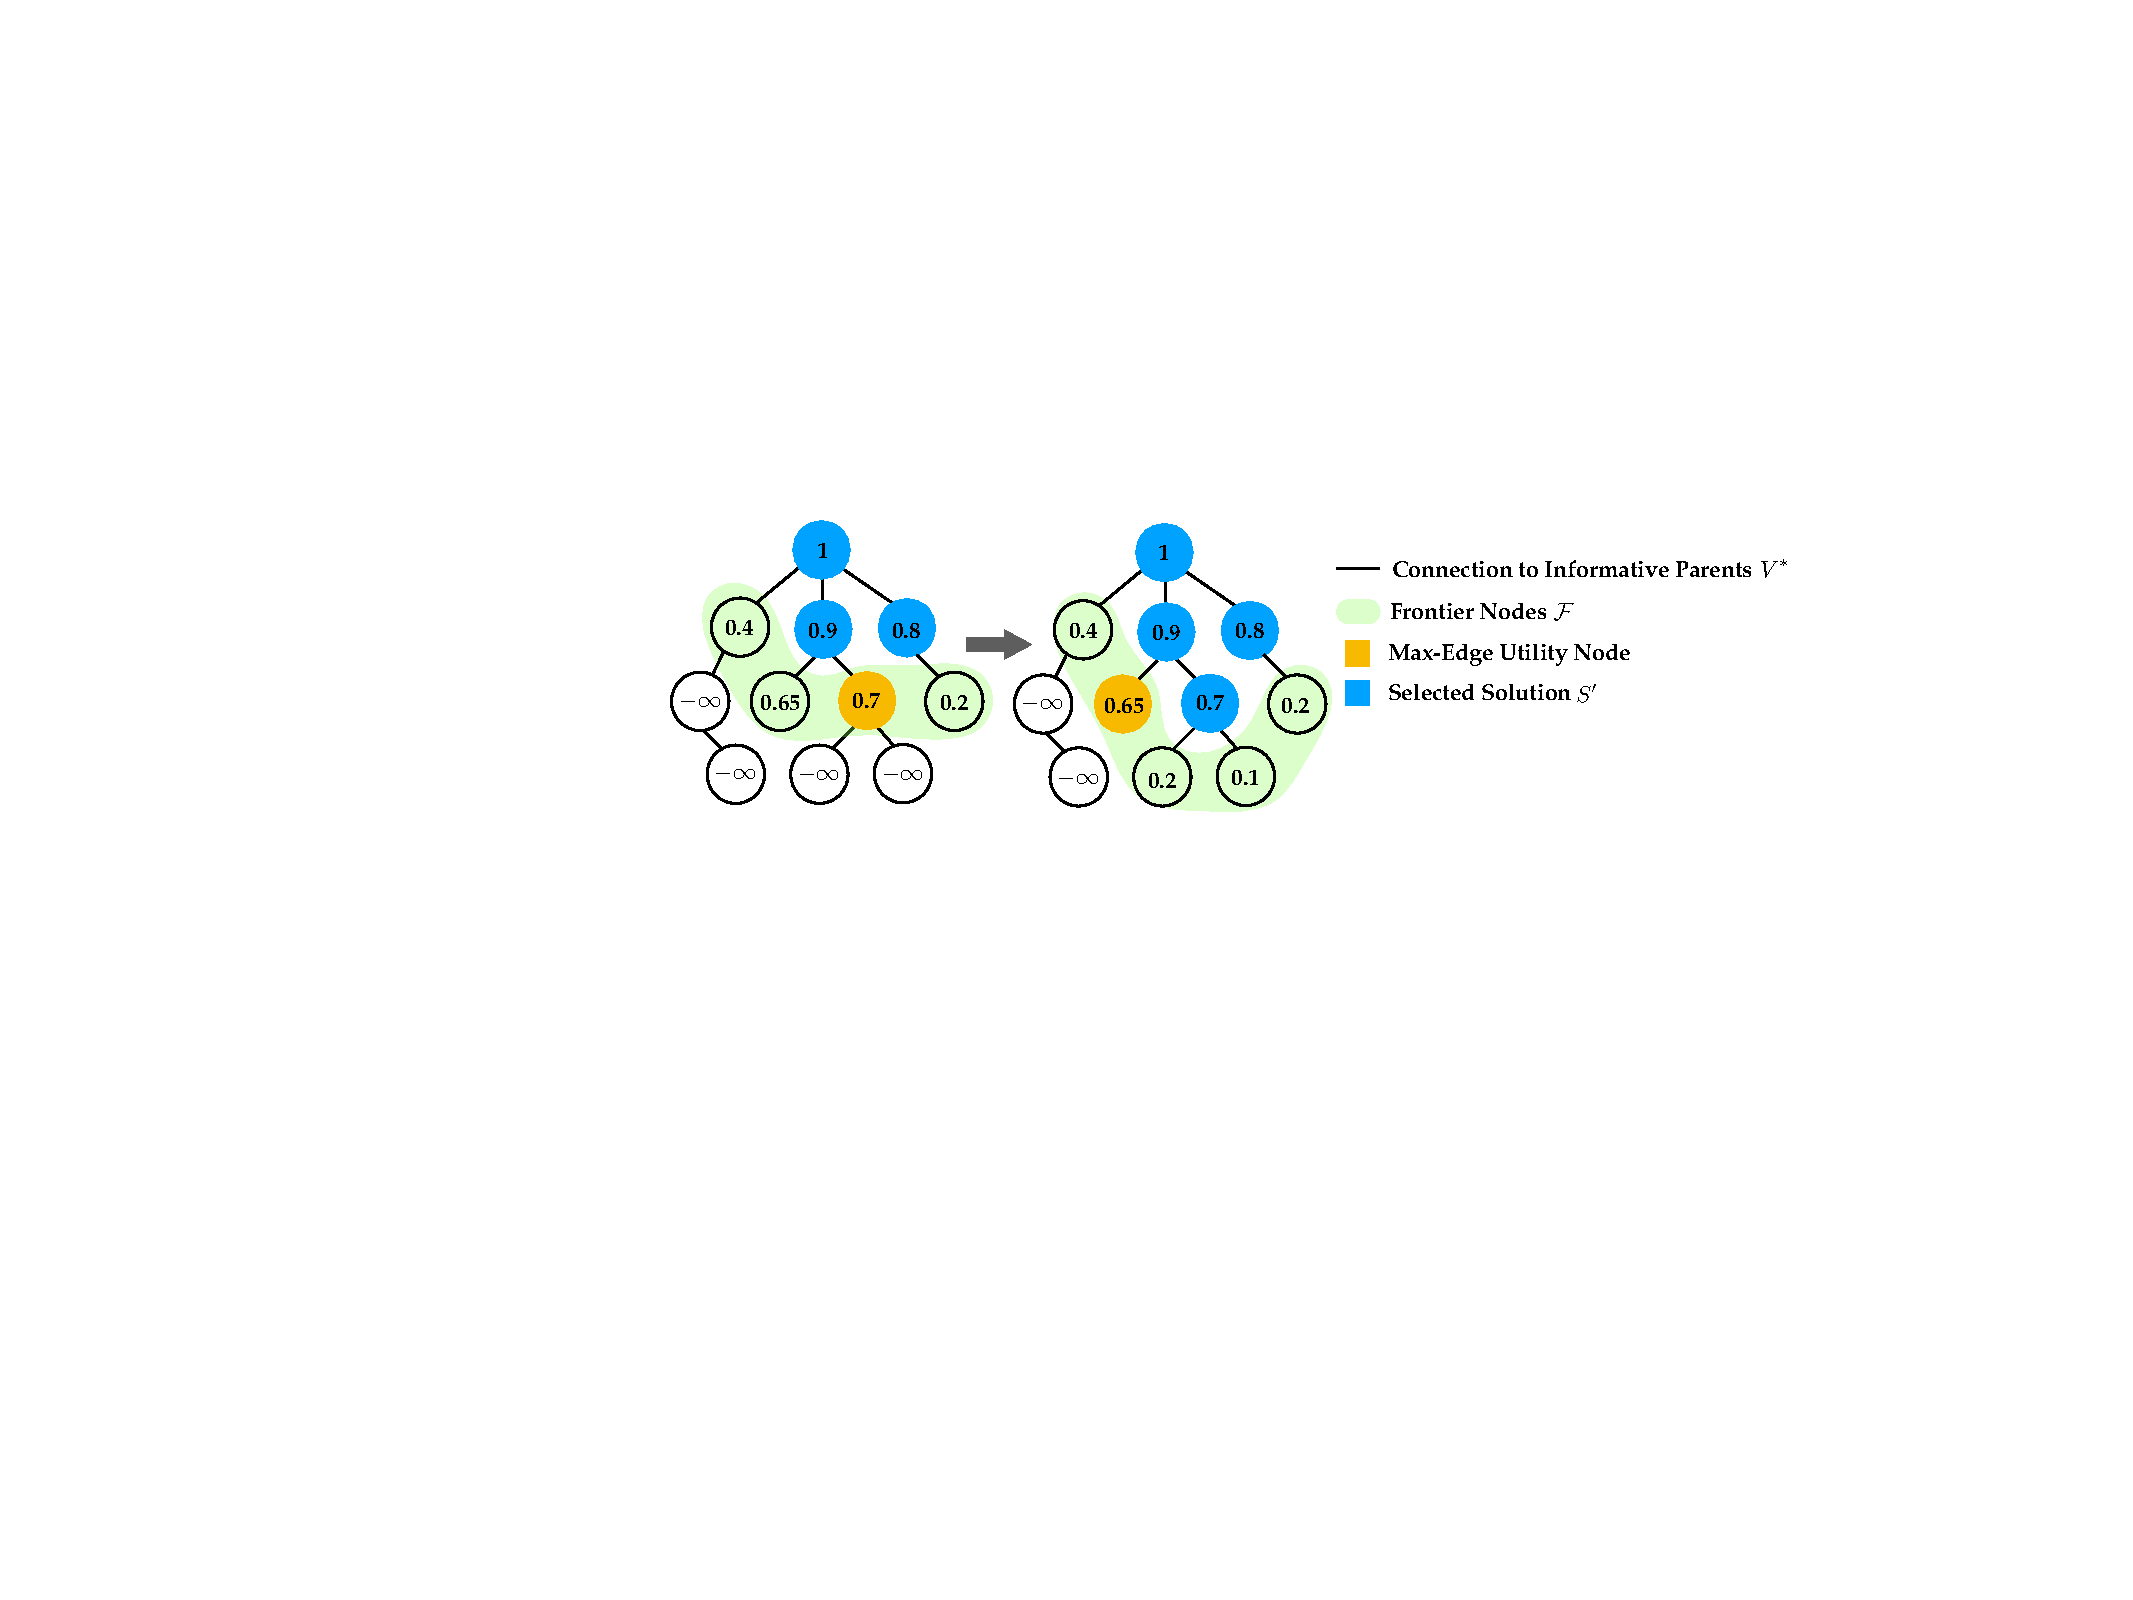
\includegraphics[width=\linewidth]{figures/frontier_greedy.pdf}
\vspace{-20pt}
\caption{Example illustrating how the frontier greedy algorithm incrementally builds up the solution by selecting the maximal-edge utility node from the frontier at every step. \achange{Starting from a pre-materialized lattice consisting of only connections to informative parents (left) and three nodes in the existing} solution (blue), we select the node with the highest edge utility \change{(yellow)} amongst the frontier nodes \change{(green)}. On the right, the newly added node results in an updated frontier and a maximum-edge utility node is selected amongst them.
\agp{I think the edge weights in the figure are really confusing. I would propose dropping it. Or, attach the utility to the nodes instead of the edges. In this case, I would say it might be interesting to set the utility of the 0.5 node to be $-\infty$ until the one with 0.4 is added first (an informative parent, perhaps). That will add to the richness of the example. Right now I can't tell if the example has edge-weights, node-weights... overall, I can't even tell what the mapping to the utility is here.}\dor{Changed.}
}
\vspace{-10pt}
\label{fig:frontier_greedy}
\end{figure}
\section{Storyboard System\label{sec:system}}
In this section, we present our system, \system, by first providing a high-level overview of the underlying algorithms, and then describing the user interaction mechanisms.
\change{
  \subsection{Lattice Traversal Algorithm\label{sec:algorithms}}
  \achange{For a given dataset and user-selected X, Ys, we first enumerating all possible attribute-value combinations (i.e. filters) to construct the lattice by  retaining only edge connections to informative parents. Now, we }discuss the algorithm used for traversing the
  lattice to select the connected subgraph $S$ of $k$
  visualizations (or equivalently, nodes in the lattice) that maximize
  the utility $U$.
}%generating the visualization lattice, and then present an overview of how we
\tr{
\stitle{Lattice Generation:} Our system supports two variants of traversal based on the lattice generation procedure---offline variants that first generate the complete lattice and then work towards identifying the solution with maximum combined-edge utility, and online variants that incrementally generate the lattice and simultaneously identify the solution. The offline variants are appropriate for datasets with a small number of low-cardinality attributes, where we can generate the entire lattice in a reasonable time; whereas the online variants are appropriate for datasets with many high-cardinality attributes, where we need to incrementally generate a partial lattice. \tr{
  To prevent the danger of visualizations with small population size, users can also select an \textit{iceberg condition} ($\delta$) to adjust the extent of pruning on visualizations whose sizes fall below a certain percentage of the overall population size. \footnote{The terminology is used in the discussion of iceberg cubes in OLAP literature~\cite{Xin2007}.}
}
%In most cases, the lattice contains a large number of visualizations due to the presence of many attributes or high-cardinality attributes in the dataset. In such cases finding an optimal solution is computationally challenging.
\stitle{Lattice Traversal:} We first describe the offline version of the algorithm before outlining the modification required for the online variant of the algorithm. Given a lattice that has been materialized offline,
}
\change{Our algorithm,
titled {\em frontier-greedy}, is inspired
\achange{by the notion of ``externals'' in Parameswaran et al.}\cite{Parameswaran2010}.
The algorithm incrementally grows a subgraph $S'$ until
$k$ nodes are selected.
Throughout, the algorithm maintains a \achange{set} of {\em frontier} nodes \achange{$\mathcal{F}$}---nodes
that are connected to the existing subgraph solution $S'$
but have not yet been
added. The frontier nodes includes all of the children of the nodes
in $S'$. \achange{Given that our pre-materialized lattice only contain edge connections to informative parents, any frontier node is guaranteed to have an informative parent in the the existing solution and can be added to $S$ without violating the informativeness principle.}
%Any frontier node whose informative parent is present in the existing solution can potentially be added to the existing solution, without violating the informativeness principle.
At each iteration, the algorithm adds the node from the frontier
nodes that leads to the greatest increase in the utility of $S'$: i.e.,
the node $V_n$ such that $U(S' \cup \{V_n\})$ is the largest.
Figure~\ref{fig:frontier_greedy} displays how the algorithm
maintains the list of frontier nodes (in green), and the current $S'$ (in blue),
adding the node that leads to the greatest increase in utility (in yellow).
Algorithm~\ref{algo:frontier_greedy} provides the pseudocode.
}
\begin{algorithm}
  \begin{algorithmic}[1]
  \Procedure{PickVisualizations}{$k$, \achange{$\mathcal{L}$}}
  \State $S' \gets$ \{$V_0$\}  \text{/* adding the overall node */}
  \While{$|S'| < k$}
      \State \achange{$\mathcal{F}$} $\gets$ getFrontier($S'$, \achange{$\mathcal{L}$})
      \State bestUtility $\gets$ $U(S')$
      \For{$\achange{V_i}$ $\in$ \achange{$\mathcal{F}$}}
      \If{$U(S' \cup \{\achange{V_i}\})>$bestUtility}
      \State maxNode $\gets$ $\achange{V_i}$
      \State bestUtility $\gets U(S' \cup \{\achange{V_i}\})$
      \EndIf
      \EndFor
      \State $S' \gets S' \cup$ \{maxNode\}
  \EndWhile
  \Return $S'$
  \EndProcedure
  \end{algorithmic}
  \caption{Frontier Greedy Algorithm\agp{The pseudocode had some inaccuracies that I tried fixing. Please carefully check.}\dor{Minor changes. Do we need to initialize maxNode in the pseudocode? For bestUtility $\gets U(S')$, would it be more clear if we initialize as bestUtility $\gets -\infty$?}}\label{algo:frontier_greedy}
\end{algorithm}
%The frontier greedy algorithm first compiles a list of candidate nodes known as the \textit{frontier} nodes, which encompasses all nodes that are connected to the existing subgraph solution. As long as the informative parents of frontier nodes are already present in the solution, the frontier nodes can be appended to the current solution without violating requirement (ii) in the problem formulation, enforcing the presence of informative parent for every selected visualization. To obtain the frontier nodes, the algorithm scans and adds all children of leaf nodes of the current dashboard as part of the frontier. \tr{In the online version, it additionally checks for each child whether its informative parent is present in the current dashboard.} As illustrated in Figure~\ref{fig:frontier_greedy}, at each step, our algorithm greedily picks the node with the maximum edge utility amongst the eligible frontier nodes to add to the current solution, and updates the frontier accordingly. \ccut{The \textit{frontier greedy} algorithm discussed here is used for generating the dashboards for our user study and we defer the details of other algorithms that we have developed for lattice traversal to the technical report. }
%\par The frontier greedy algorithm obtains a list of candidate nodes known as the \textit{frontier} nodes, which encompasses all neighbors of nodes in the existing subgraph solution. Any of the nodes in the frontier can be added to the current solution since their informative parent is present in the solution. To obtain the frontier nodes, the algorithm scans and adds all children of leaf nodes of the current dashboard as part of the frontier. In the online version, it additionally checks for each child whether its informative parent is present in the current dashboard. At each step, our algorithm greedily picks the node with the maximum utility amongst the frontier nodes to add to the current solution, and updates the frontier accordingly. \tr{The path merging algorithm first generate the informative paths from root to every candidate node. Then, it greedily merges the paths with high-utility to create a subgraph whose size is less than or equal to maximum capacity $k$.}

\subsection{User Interaction\label{sec:interaction}}
\begin{figure*}[ht!]
\centering
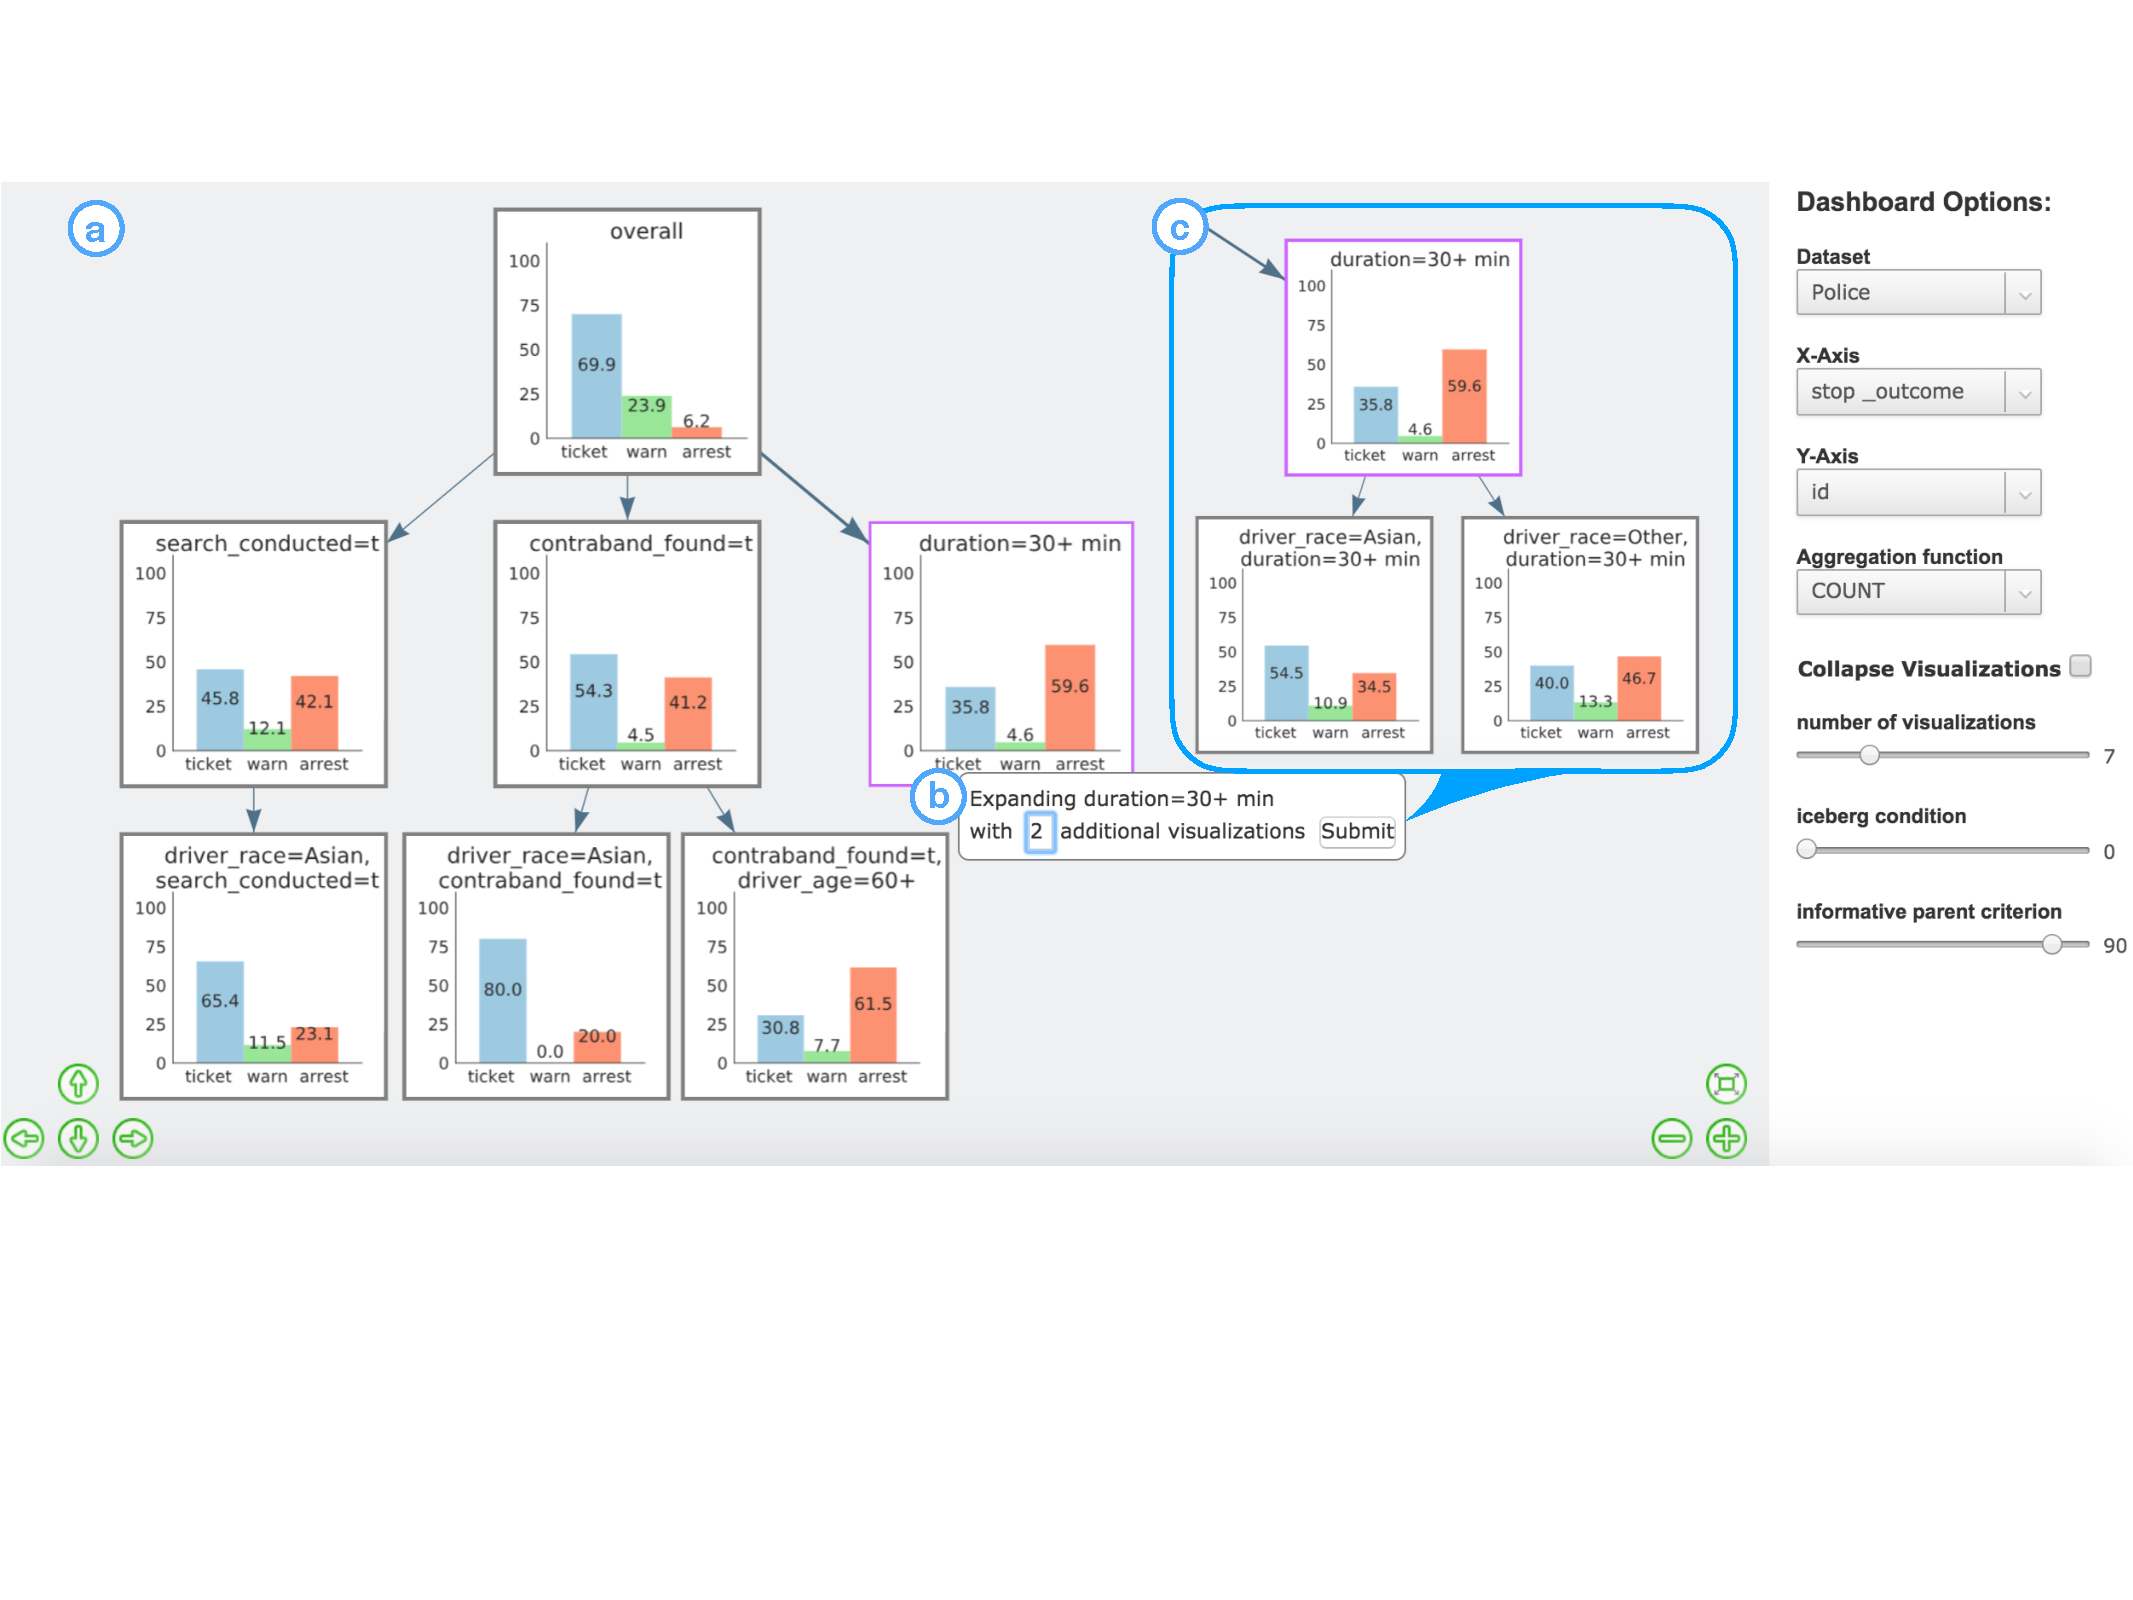
\includegraphics[width=0.9\linewidth,frame]{figures/overview_interface_expand.pdf}
\caption{a) Overview of the \system interface for the Police Stop dataset. Users can  select \change{x, y axes, and aggregation function via the dropdown menu, to define the visualization space of interest, as well as adjusting dashboard parameters, such as the number of visualizations to show in the dashboard (k) via the sliders.} b) User clicks on the duration=30+min visualization to request 2 additional visualizations. c) A preview of the added portion of the resulting dashboard is shown.}
% Default values are set for system related parameters such as the number of visualizations to show in the dashboard (k), iceberg condition for pruning ($\delta$), and informative parent criterion ($\theta$), which can be adjusted by the users via the sliders if needed.
\label{fig:overview}
\vspace{-10pt}
\end{figure*}%optional system parameter settings

\change{Given the visualizations in $S'$,
we can render these visualizations in a dashboard,}
where users can inspect the \change{visualizations}
through panning and zooming with navigation buttons,
mouse clicks, and key bindings.
Users can also select the x and y axes of interest,
aggregation function, and \change{set the number of visualizations ($k$)}
to generate a dashboard.
\change{Figure~\ref{fig:overview} displays
\system in action on the Police stop dataset~\cite{police}.
}
The dataset contains records of vehicle and pedestrian stops from law enforcement departments in Connecticut, dated from 2013 to 2015. In this case, the analyst is interested in the percentages of police stops \change{(Y)} that led to different outcomes \change{(X)}, such as ticket, warning, or arrest.
\change{As shown in Figure \ref{fig:overview}a, the analyst
may begin by generating a 7-visualization dashboard.
\achange{She} would learn that if a search is conducted (\texttt{search\_conducted=t}),
then the probability of being arrested increases from \achange{6.2\% to 42.1\%}.
However, the probability goes down to \achange{23.1\%}
if the driver is Asian (\texttt{driver\_race=Asian, search\_conducted=t}).
When examining these visualizations, the analyst can be confident that
any deviations are both informative and interesting: that is, the informative
parents are present for each child,
making the takeaways more significant.
Moreover,
the analyst may learn that for drivers
who had contraband found in the vehicle (\texttt{contraband\_found=t}),
the arrest rate for those who are 60
and over is surprisingly higher than usual,
whereas for Asian drivers the arrest rate is lower.
}

After browsing through visualizations in the dashboard,
\achange{the analyst} may be interested in getting more information
about a specific visualization.
\system allows \achange{analysts} \change{to perform additional
drill-downs by requesting}
a new dashboard centered on a chosen visualization
of interest as the new starting point
(or equivalently, the root of the lattice)
for analysis.
Say the analyst is now interested in learning more
about the other factor that contributes to \achange{high arrest rates}:
\change{a long stop with \texttt{duration=30+min}}.
In Figure~\ref{fig:overview}b, \achange{she}
can click on the corresponding visualization
\change{to} request additional visualizations.
Upon seeing the updated dashboard in Figure~\ref{fig:overview}c,
she learns that any visualization
that involves the \change{\texttt{duration=30+min}}
filter is likely to result in high ticketing and arrest rates.
This implies that if a police stop lasts more than 30 minutes,
the outcome would more or less be the same,
independent of other factors such as the driver's race or age.
To generate the expanded dashboard, \system uses the same models
and algorithms as before,
except the \achange{the overall visualization $V_0$ at the root node is now set as the selected visualization}.
This node expansion capability is motivated
by the idea of \textit{iterative view refinement}
\change{common in other} visual analytics systems,
which is essential for users to iterate on and
explore different hypotheses~\cite{Hoque2017,Wongsuphasawat2016}.

%!TEX root = main.tex
\change{\section{Evaluation Study Methods\label{sec:userstudy}}}
%between-subject
In this section, we describe the methodology
for \change{a user study}
we conducted for evaluating the
\change{usefulness of \system
for various exploratory analysis tasks}.
We aim to evaluate whether \change{\system's ``3S'' design principles enables analysts }to effortlessly identify insights in comparison
with \change{conventional approaches for multidimensional data exploration}.%other dashboard generation baselines
\subsection{\change{Participants and Conditions}}
We recruited 18 participants \change{(10 Male; 8 Female)}
with prior experience in working with data.
Participants included undergraduate
and graduate students, researchers,
and data scientists, with $1-14$ years of data
analysis experience (average: $5.61$).
\tr{This can include, but are not limited to, browsing and reading data, data cleaning and wrangling, data visualization and model building. The inclusion criteria is assessed based on a self-reporting basis in the pre-study survey.}
No participants reported prior experience
in working with the two datasets used in the study (described below).
Participants were randomly assigned two
of the three types of dashboards with \change{$k=10$}
visualizations generated \change{via the}
following conditions.
\papertext{\change{The specific dashboards for each dataset and condition can be found in our technical report~\cite{TR}}.}
%(described in Section \ref{sec:algorithms})
\stitle{\system:} The dashboards for this condition
are generated by the aforementioned
frontier greedy algorithm and displayed
in a hierarchical layout as in Figure~\ref{fig:overview}.
\cut{To ensure the informativeness of the generated dashboards,
we selected a more stringent $\theta$=90\%
criteria to generate the dashboards for our user study.}
To establish a fair comparison
with the two other conditions,
we deactivated \cut{iceberg pruning (by setting $\delta$=0) and}
the interactive node expansion capabilities.
\stitle{\BFS (short for breadth-first search):}
Starting from the visualization of the \change{overall} population,
$k$ visualizations are selected level-wise,
traversing down the subset lattice,
adding the visualizations at the first level
with $1$-filter combination one at a time,
\change{and then visualizations with $2$-filter combinations},
and so on,
until $k$ visualizations have been added.
This baseline is designed to simulate a dashboard
generated by a meticulous analyst who exhaustively
inspects all visualizations (i.e., filter combinations)
from the top down.
\change{These visualizations are then displayed
in a $5\times2$ table.}
\stitle{\cluster:} \change{In this condition,}
$k$-means clustering is first performed on the data distributions
\change{of all of the visualizations in the lattice}.
This results in $k$ clusters \change{that cover the rest of the}
visualizations.
\change{For each cluster, we select
the visualization with the least number of filter conditions
as the cluster representative for interpretability}\tr{\footnote{Since the clusters cover all visualizations in the dataset and the overall visualization has the minimum number of filter across all visualization, the overall visualization is guaranteed to be picked as one of the displayed visualizations.}}
and display them in a $5\times2$ table layout.
This baseline is designed to showcase a diverse set of
distributions within the dataset.
\tr{
  \begin{figure*}[ht!]
  \centering
  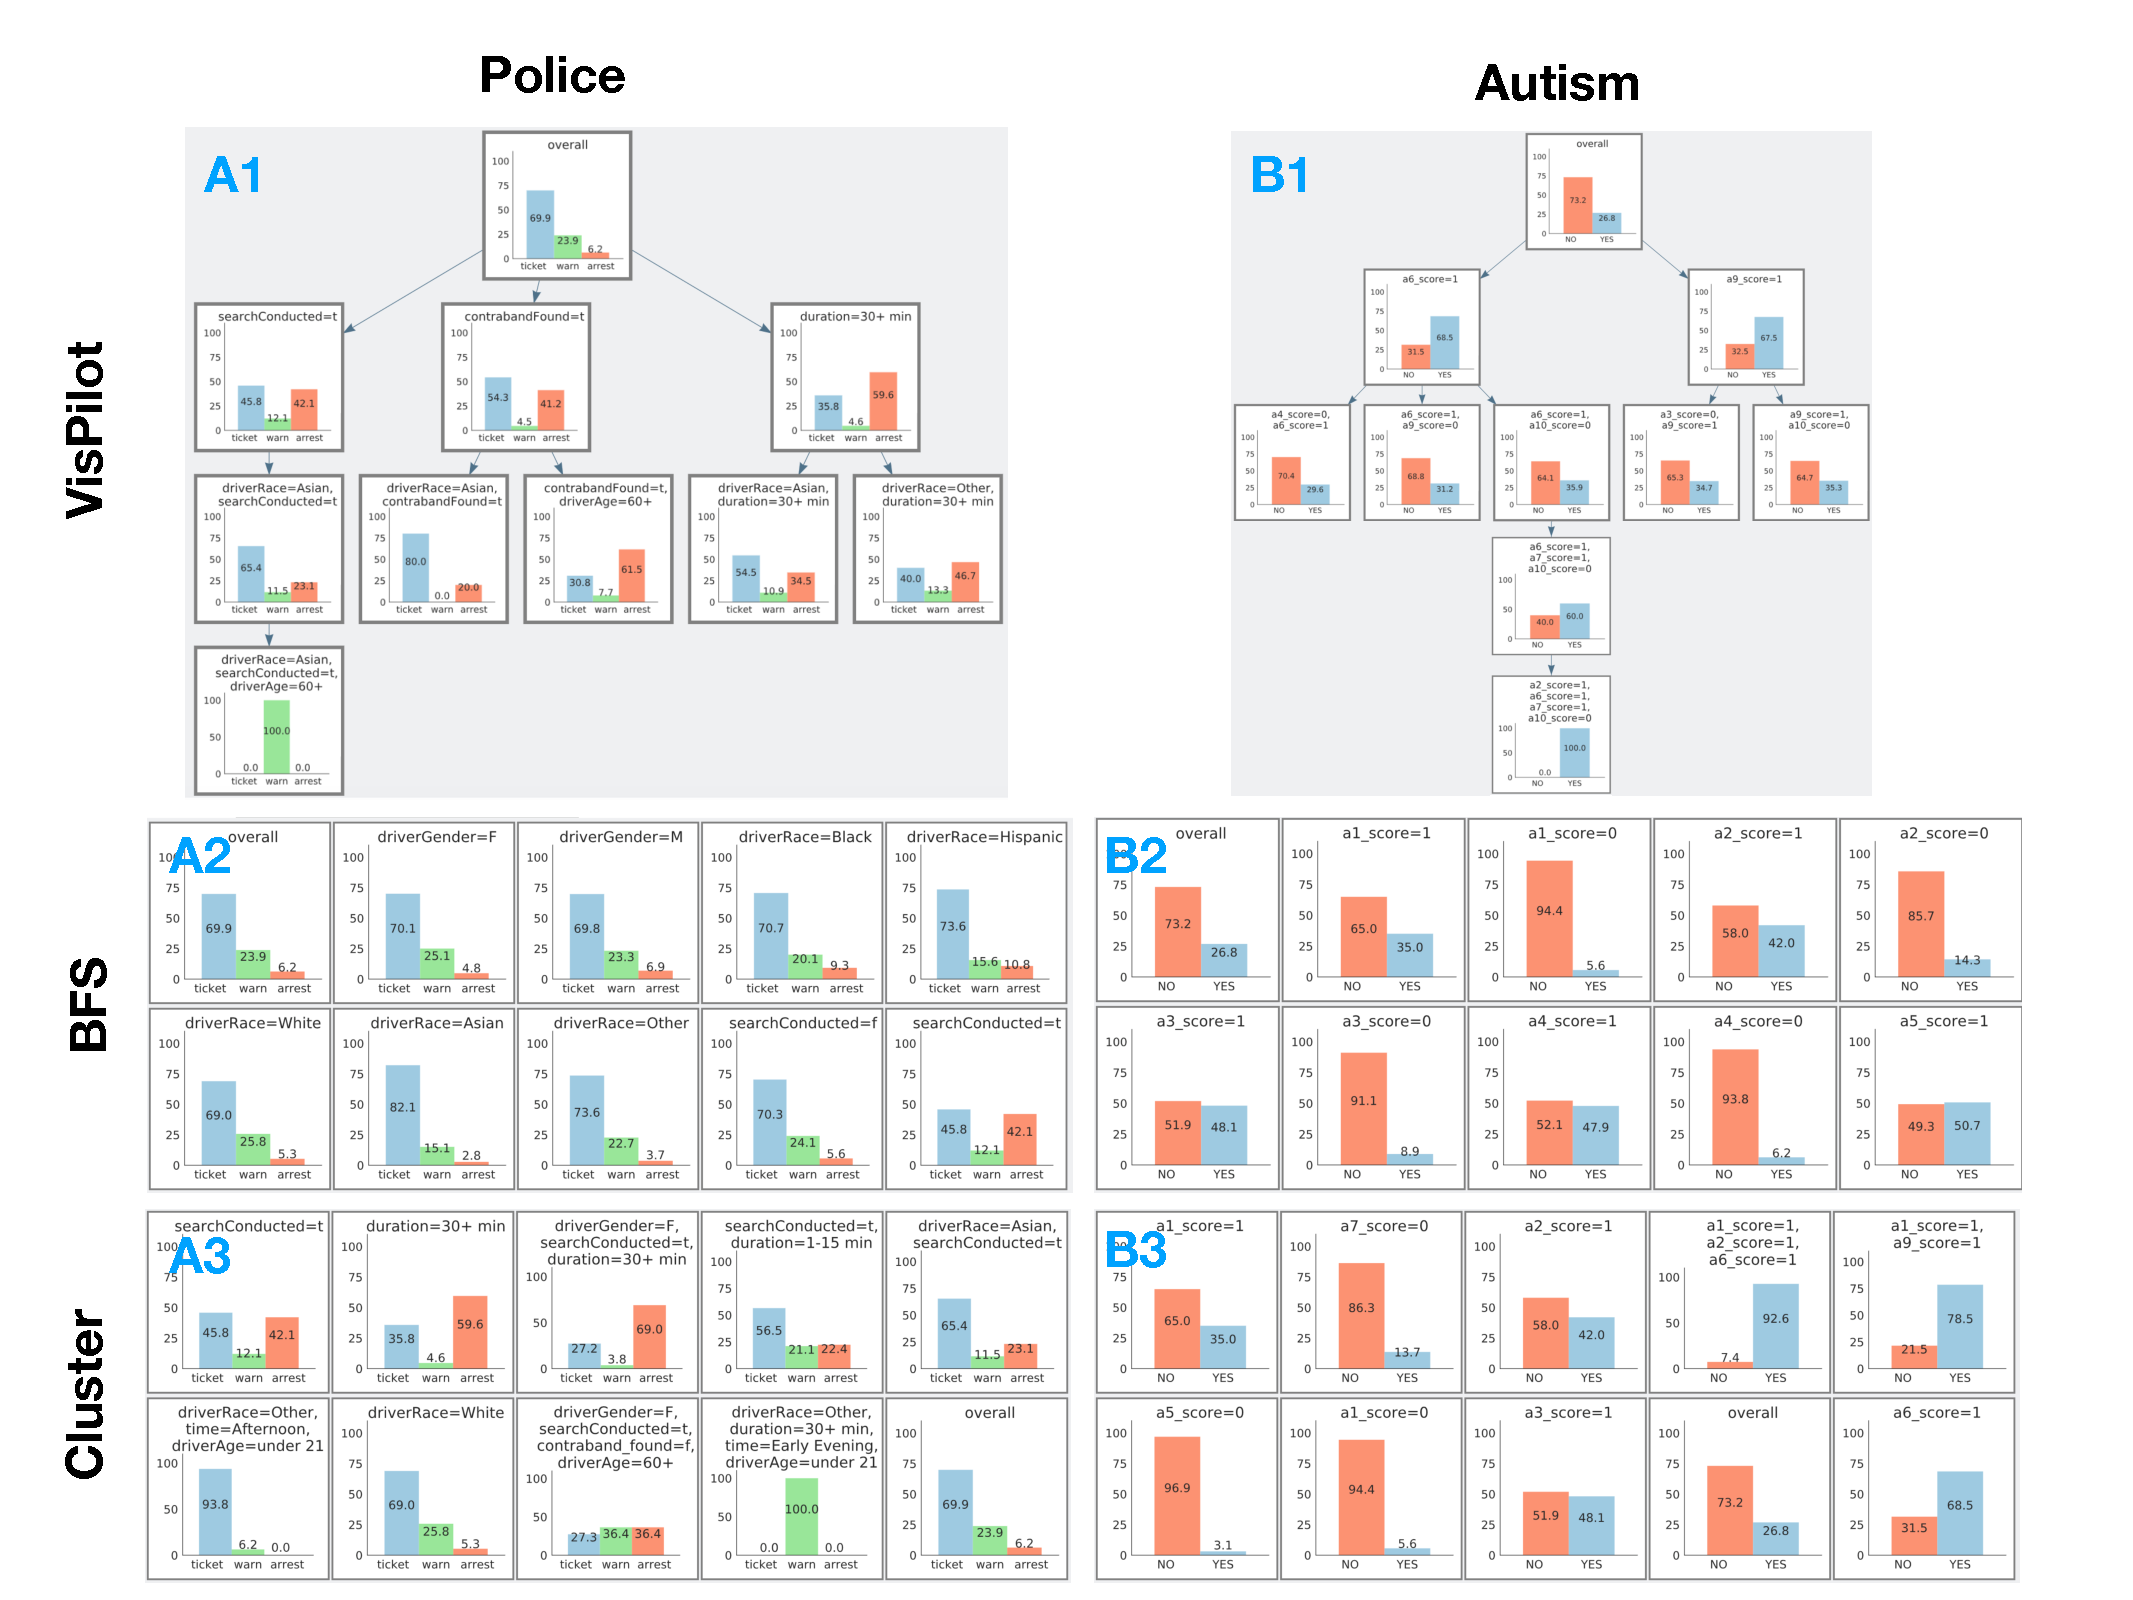
\includegraphics[width=0.95\linewidth]{figures/dashboard_examples.pdf}
  \caption{\tr{Specific dashboards for each dataset and condition used in the study.}}
  \label{fig:dashboards}
  \vspace{-10pt}
  \end{figure*}
}
\smallskip
\stitle{Dataset Descriptions.}
Each participant was assigned two different
conditions on two different datasets
\change{(Police Stop and Autism, described below)}.
The ordering of each condition was
randomized to prevent confounding learning effects.
The study began with a 5-minute tutorial
using dashboards generated from the Titanic dataset~\cite{titanic}
for each condition.
To prevent bias across conditions,
participants were not provided an explanation of
how the dashboards were generated and
why the visualizations were arranged in a particular way.

\change{The first dataset in the study} was the aforementioned
Police Stop dataset.
The attributes in the dataset
include driver gender, age, race, stop time of day,
stop outcome, whether a search was conducted,
and whether contraband was found.
We generated dashboards of bar chart visualizations
with x-axis as the stop outcome
(i.e., whether the police stop resulted in a
ticket, warning, or arrest) and y-axis as the percentage of police stops that led to each outcome. %We randomize the ordering for each task combination to prevent confounding learning effects. %%, which contains visualizations of the \% of police stop that resulted in a warning, ticket, or an arrest. %, which contains a total of 312948 records of vehicle and pedestrian stops from law enforcement departments in Connecticut, dated from 2013 to 2015.

The second dataset in the study
was the Autism dataset~\cite{autism},
\change{describing} the results of autism spectrum
disorder screening for 704 \change{adults}.
The attributes in the dataset are binary responses
to 10 diagnostic questions
as part of the screening process.
This dataset serves as a data-agnostic condition,
since there was no descriptions
of the questions or answer labels provided to
\change{our study participants}.
We generated dashboard visualizations
based on \change{the percentage of adults that were diagnosed with autism}.

\change{\subsection{Study Procedure}
\par After the tutorial, for each dataset, participants}
were given some time to read through a worksheet
containing the descriptions of the data attributes.
Then, they were given an attention check question
where they were
\change{provided}
a verbal description of the visualization filter
\change{(i.e., data subset)}
and asked about the corresponding visualization in the dashboard.
After understanding the dataset and chart schema,
participants were asked to accomplish
\change{various
tasks.
Since \system was developed
based on a joint utility objective,
it is impossible to design tasks that evaluate
each of the ``3S'' principles individually.
Instead, our tasks were selected to measure
the overall efficacy and usefulness
of the dashboards
in helping a participant
understand and become aware of different aspects of
and insights within a dataset
during drill-down analysis.
These different aspects of
dataset understanding
can be roughly illustrated
via Figure~\ref{fig:frontier_greedy},
from insights
gained from \emph{individual}
displayed visualizations (blue selected nodes),
to predicting behavior of \emph{related}
visualizations (green related nodes),
to understanding \emph{overall} attribute importance
(entire lattice, a mix of green, blue, and unselected white nodes).
}

\stitle{\change{Labeling (Individual Assessment):}}
Participants were asked to talk aloud
as they interpreted the visualizations
in the dashboard and \change{label}
each one as interesting or
not interesting, \change{or leave it unselected}.
This \change{subjective task measures}
how \change{interesting \emph{individual}
selected visualizations were}
to participants. % (RQ\change{1}).%well are participants at retrieving interesting visualizations (RQ1).
\stitle{\change{Prediction (Related Assessment):}}
Participants were given a separate worksheet
and asked to sketch an estimate for a visualization
that is not present in the dashboard.
For every condition, the visualization to be estimated
contained $2$ filter combinations,
with exactly one parent present in the given dashboard.
After making the prediction,
participants were shown the actual data
distribution and asked to rate on a Likert scale
of 10 how surprising the result was
\change{(1: not surprising and 10: very surprising)}.
\change{This task measured how well participants
inferred the behavior of \emph{related},
unobserved visualizations based on a
limited set of selected dashboard visualizations.}
\stitle{\change{Ranking (Overall Assessment):}}
Participants were given a sheet of paper
with all the attributes listed
and asked to rank the attributes
in order of importance in contributing
to a particular outcome
(e.g., factors leading to an arrest or autism diagnosis).
Participants were allowed to assign equal ranks to more than one attribute or skip attributes that they were unable to infer importance for.
Attribute ranking tasks are \change{common in many data science
use-cases, such as feature selection and key driver analysis. Since all dashboards were equal in size, our goal was to check whether this size limitation came at the cost of \emph{overall} dataset understanding. Thus, the goal of this task was to study participant's overall dataset understanding by measuring how well participants judged the relative importance of each attribute.}% in contributing towards an outcome. %(RQ3).
 %(RQ2).}
%\change{This task measured how \emph{informative} the displayed visualizations are in allowing participants to predict unseen visualizations.}
\smallskip
\par At the end of the study, we asked two open-ended questions regarding the insights \change{gained by} participants and what they \change{liked or disliked} about each dashboard. On average, the study lasted around 48 minutes.
%\agp{Order of RQs here and in study results are different. The way the RQs are described are different as well. Please fix before I look at S5}\dor{Earlier, we arranged the results in S5 in the chronological order in which it was conducted through the study, but the interestingness task is the most subjective and underwhelming result, so we instead focus on the informative task first as RQ1 to reinforce the connection with drill-down fallacy. I've changed the RQ labels in S4 to fit this, albeit still a bit awkward in S4.}

%!TEX root = main.tex

	\section{Study Results}
	\change{
	 We introduce the study findings for each task starting from the narrowest scope of \emph{individual} visualizations to the widest scope of \emph{overall} dataset understanding.
}
\change{\stitle{RQ1: How are \emph{individual} selected visualizations in the dashboard perceived subjectively by the users?}
}
\npar Using click-stream data logged from the user study,
we recorded whether a
participant \change{labeled each} visualization
in the dashboard as interesting, not interesting,
or left the visualization unselected.
Table~\ref{table:interestingScore} summarizes
\change{the} counts of visualizations
marked as interesting or not interesting
aggregated across conditions.
We also normalize the interestingness count
by the total number of selected visualizations
to account for variations in how some participants
select more visualizations than others.
The results indicate that participants who
used \system\ \change{saw} more
visualizations that they found interesting compared
to the \BFS and \cluster \change{\xspace conditions}.
\change{While  \change{this task is
inherently subjective, with many possible
reasons why a participant may have marked a visualization
as interesting, this result is indicative of the fact that the
selected visualizations were deemed to be relevant
by users. We will drill into \achange{the} possible reasons why in the next section.}}
\begin{table}[h!]
\vspace{-5pt}
	\centering
	\begin{tabular}{lrrr}
	 \small{Condition}             &   \small{\system} &   \small{\BFS} &   \small{\cluster} \\
	\hline
	 \small{Interesting}            &  \cellcolor{blue!25}       66    & 61    &      51   \\
	 \small{Not Interesting}        &  \cellcolor{blue!25}       10    & 20    &      22   \\
	 \small{Interesting (Normalized)} &   \cellcolor{blue!25}       0.87 &  0.75 &       0.7 \\
	\end{tabular}
	\caption{Total counts of visualizations marked as interesting or not interesting across the different conditions. \system leads to more visualizations marked as interesting and fewer visualizations marked as uninteresting.}
	\label{table:interestingScore}
	\vspace{-20pt}
\end{table}
\stitle{\change{RQ2: How well do dashboard visualizations provide users with an accurate \change{understanding} of \emph{related} visualizations?}}
\npar
\change{As discussed in Section~\ref{sec:problem},
contextualizing visualizations correctly with informative
references can help prevent users from falling prey to
drill-down fallacies. To this end,
the prediction task aims to assess whether
users can employ visualizations in the dashboard
to correctly predict unseen ones.
Indeed, if the dashboard is constructed well,
one would expect that \achange{ visualizations}
that are not very surprising relative to their informative parents
would be excluded from the dashboard
(i.e., their deviation from their informative parents is not large).}
\begin{figure}[h!]
\centering
\vspace{-10pt}
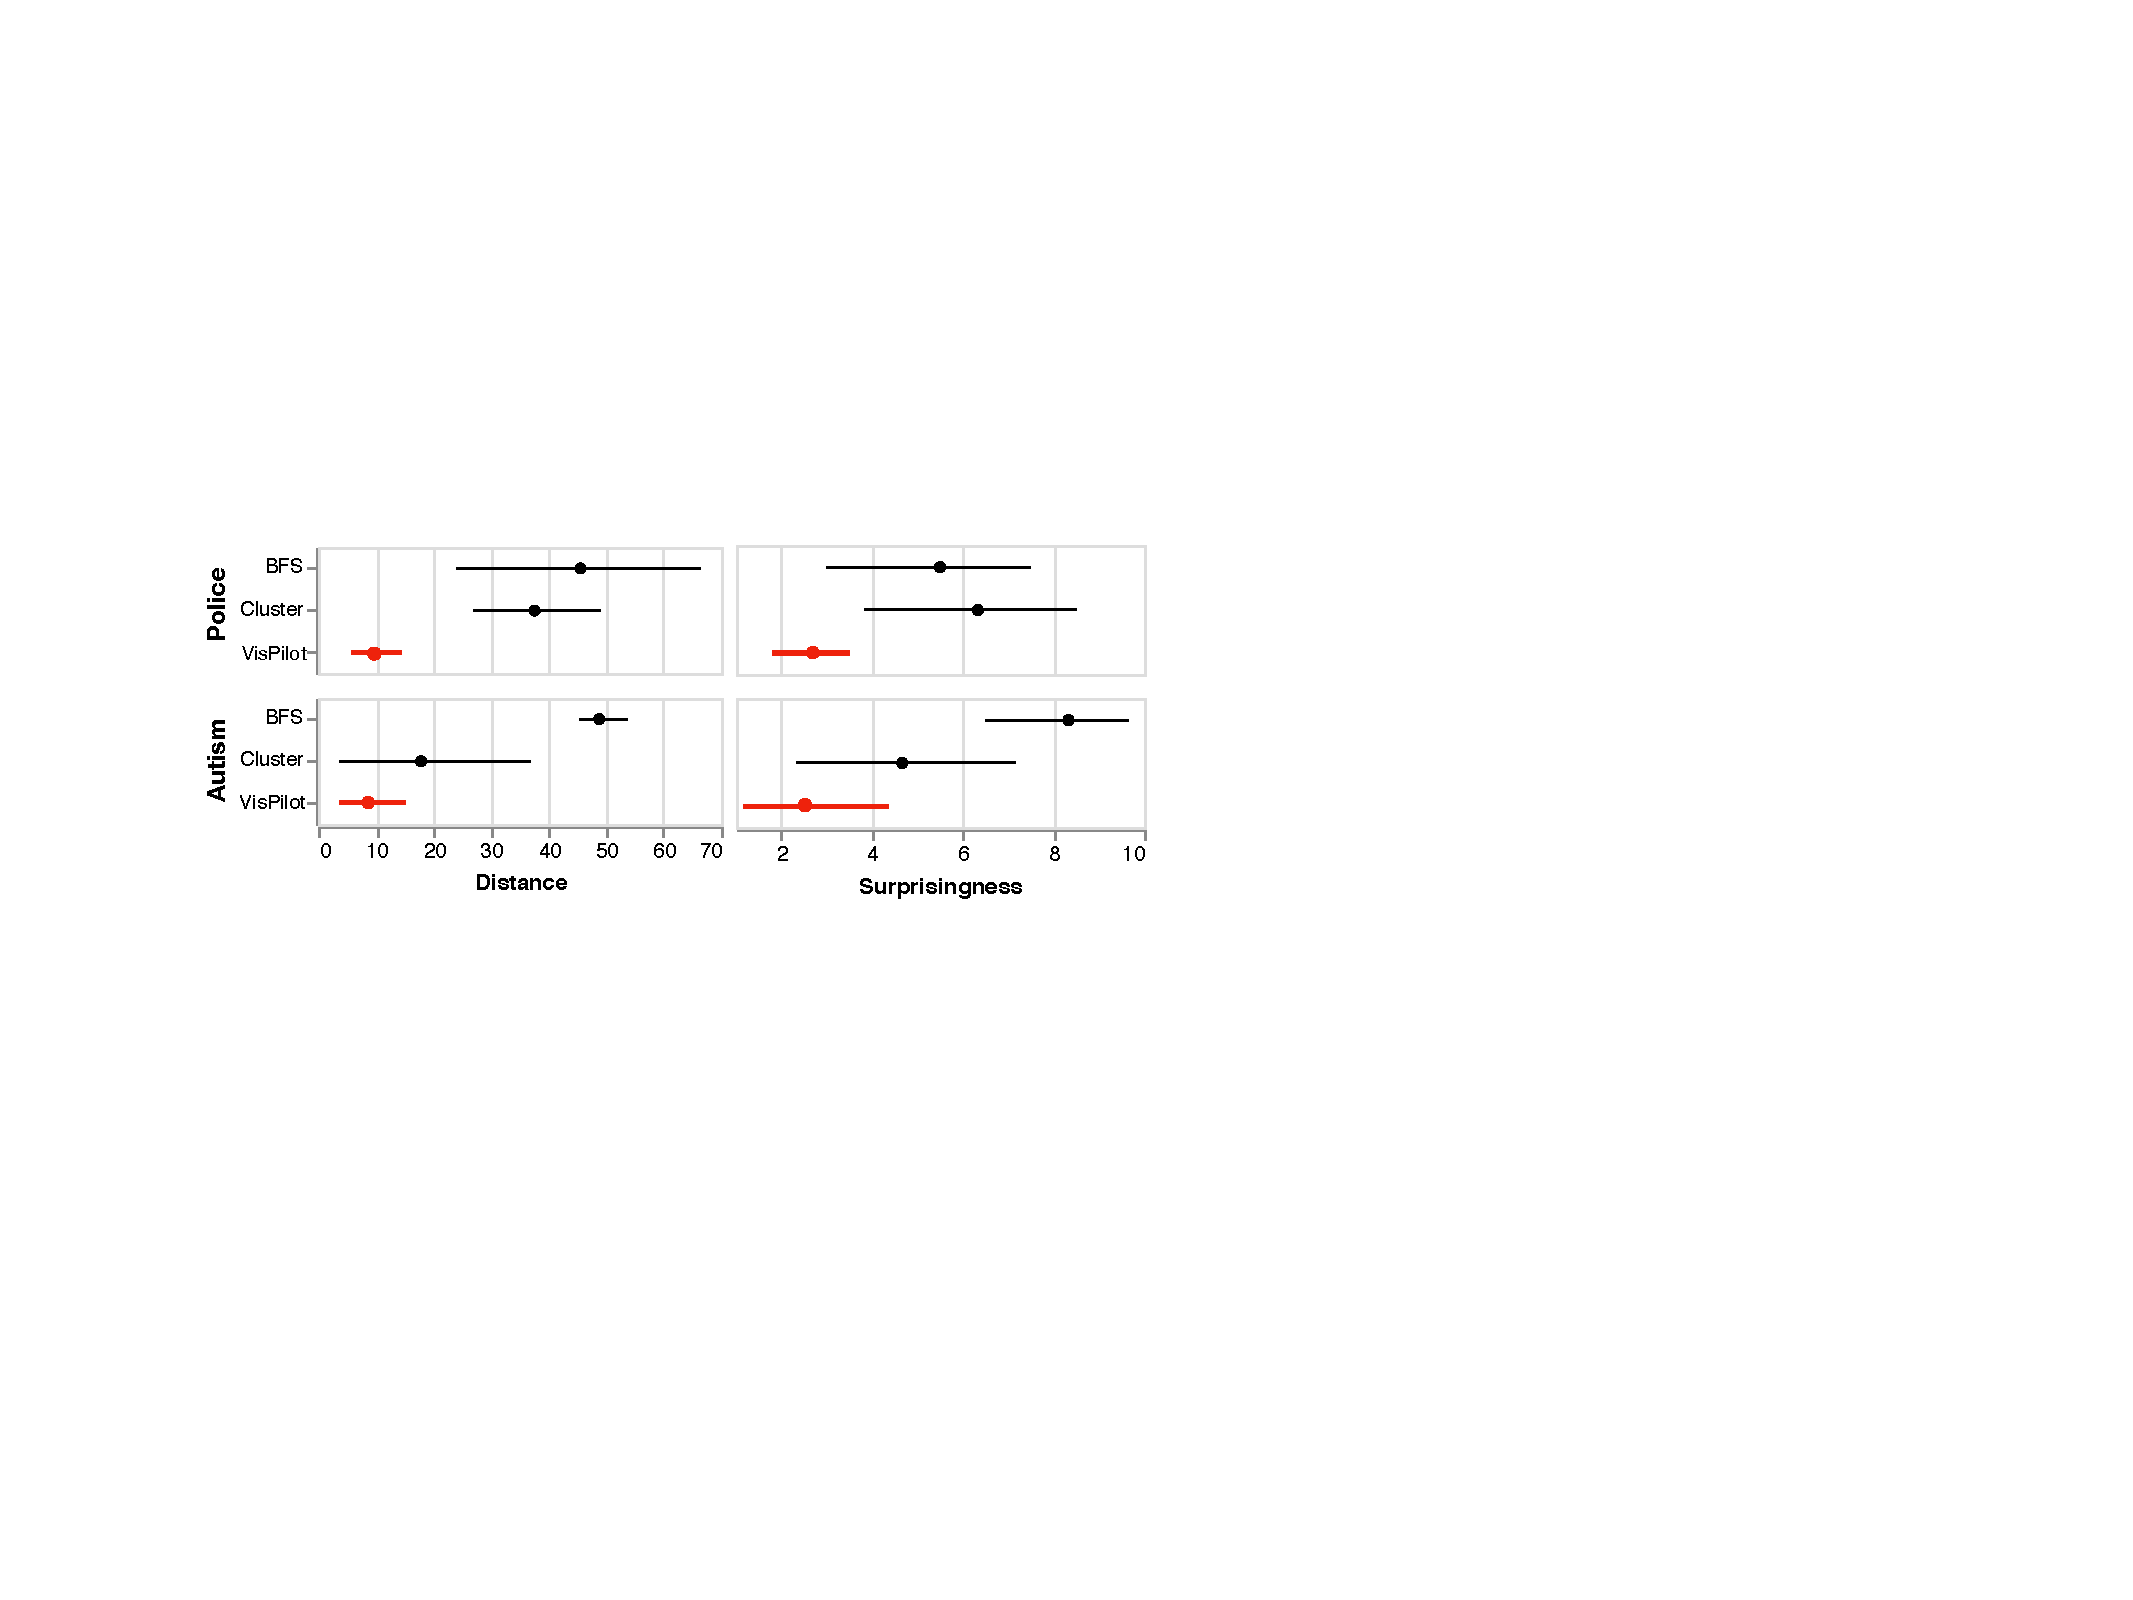
\includegraphics[width=0.95\linewidth]{figures/prediction_surprisingness_distance.pdf}
\vspace{-5pt}
\caption{Left: Euclidean distance between predicted and ground truth. In general, predictions made using \system are closer to ground truth. Right: Surprisingness rating reported by users after seeing the actual visualizations on a Likert scale of 10. \system participants had a more accurate mental model of the unseen visualization and therefore reported less surprise than compared to the baselines.}
\vspace{-10pt}
\label{fig:distance}
\end{figure}
\par The accuracy of participants' predictions
\change{is measured using}
the Euclidean distance between \change{their} predicted distributions and ground truth data distributions.
As shown in Figure~\ref{fig:distance} (left),
predictions made using \system\ (highlighted in red)
were closer to the actual distribution than compared to the baselines,
as indicated by the smaller Euclidean distances.
Figure~\ref{fig:distance} (right) also shows
that \system participants \change{were able to more
accurately reason about the expected properties of
unseen data subsets \change{(or visualizations)},
since they rated the resulting visualizations to be less surprising}.
\cluster may have performed better \change{for}
the Police dataset than it did \change{for}
the Autism \change{one},
\change{for the same reason as in the attribute ranking task,
where more univariate visualizations happened to be selected\achange{.}}%,described subsequently.


\par We also compute the variance of participants' predictions across the same condition. In this case, low variance implies
that \change{there is consistency or agreement between the predictions of participants
who consumed the same dashboard},
whereas high variance implies that the
dashboard did not convey a clear data-driven story
that could guide participants' predictions.
So instead, participants \change{had to rely on prior knowledge or} guessing to
\change{inform} their \achange{predictions}. These trends can be observed in both Figure~\ref{fig:distance} and in more detail in Figure \ref{fig:actual_predictions}, where the prediction variance amongst participants who used \system\ is generally lower than the variance for the baselines. \change{Overall, \system provides participants with a more accurate and consistent model of \emph{related} visualizations.}
\begin{figure}[h!]
\vspace{-10pt}
\centering
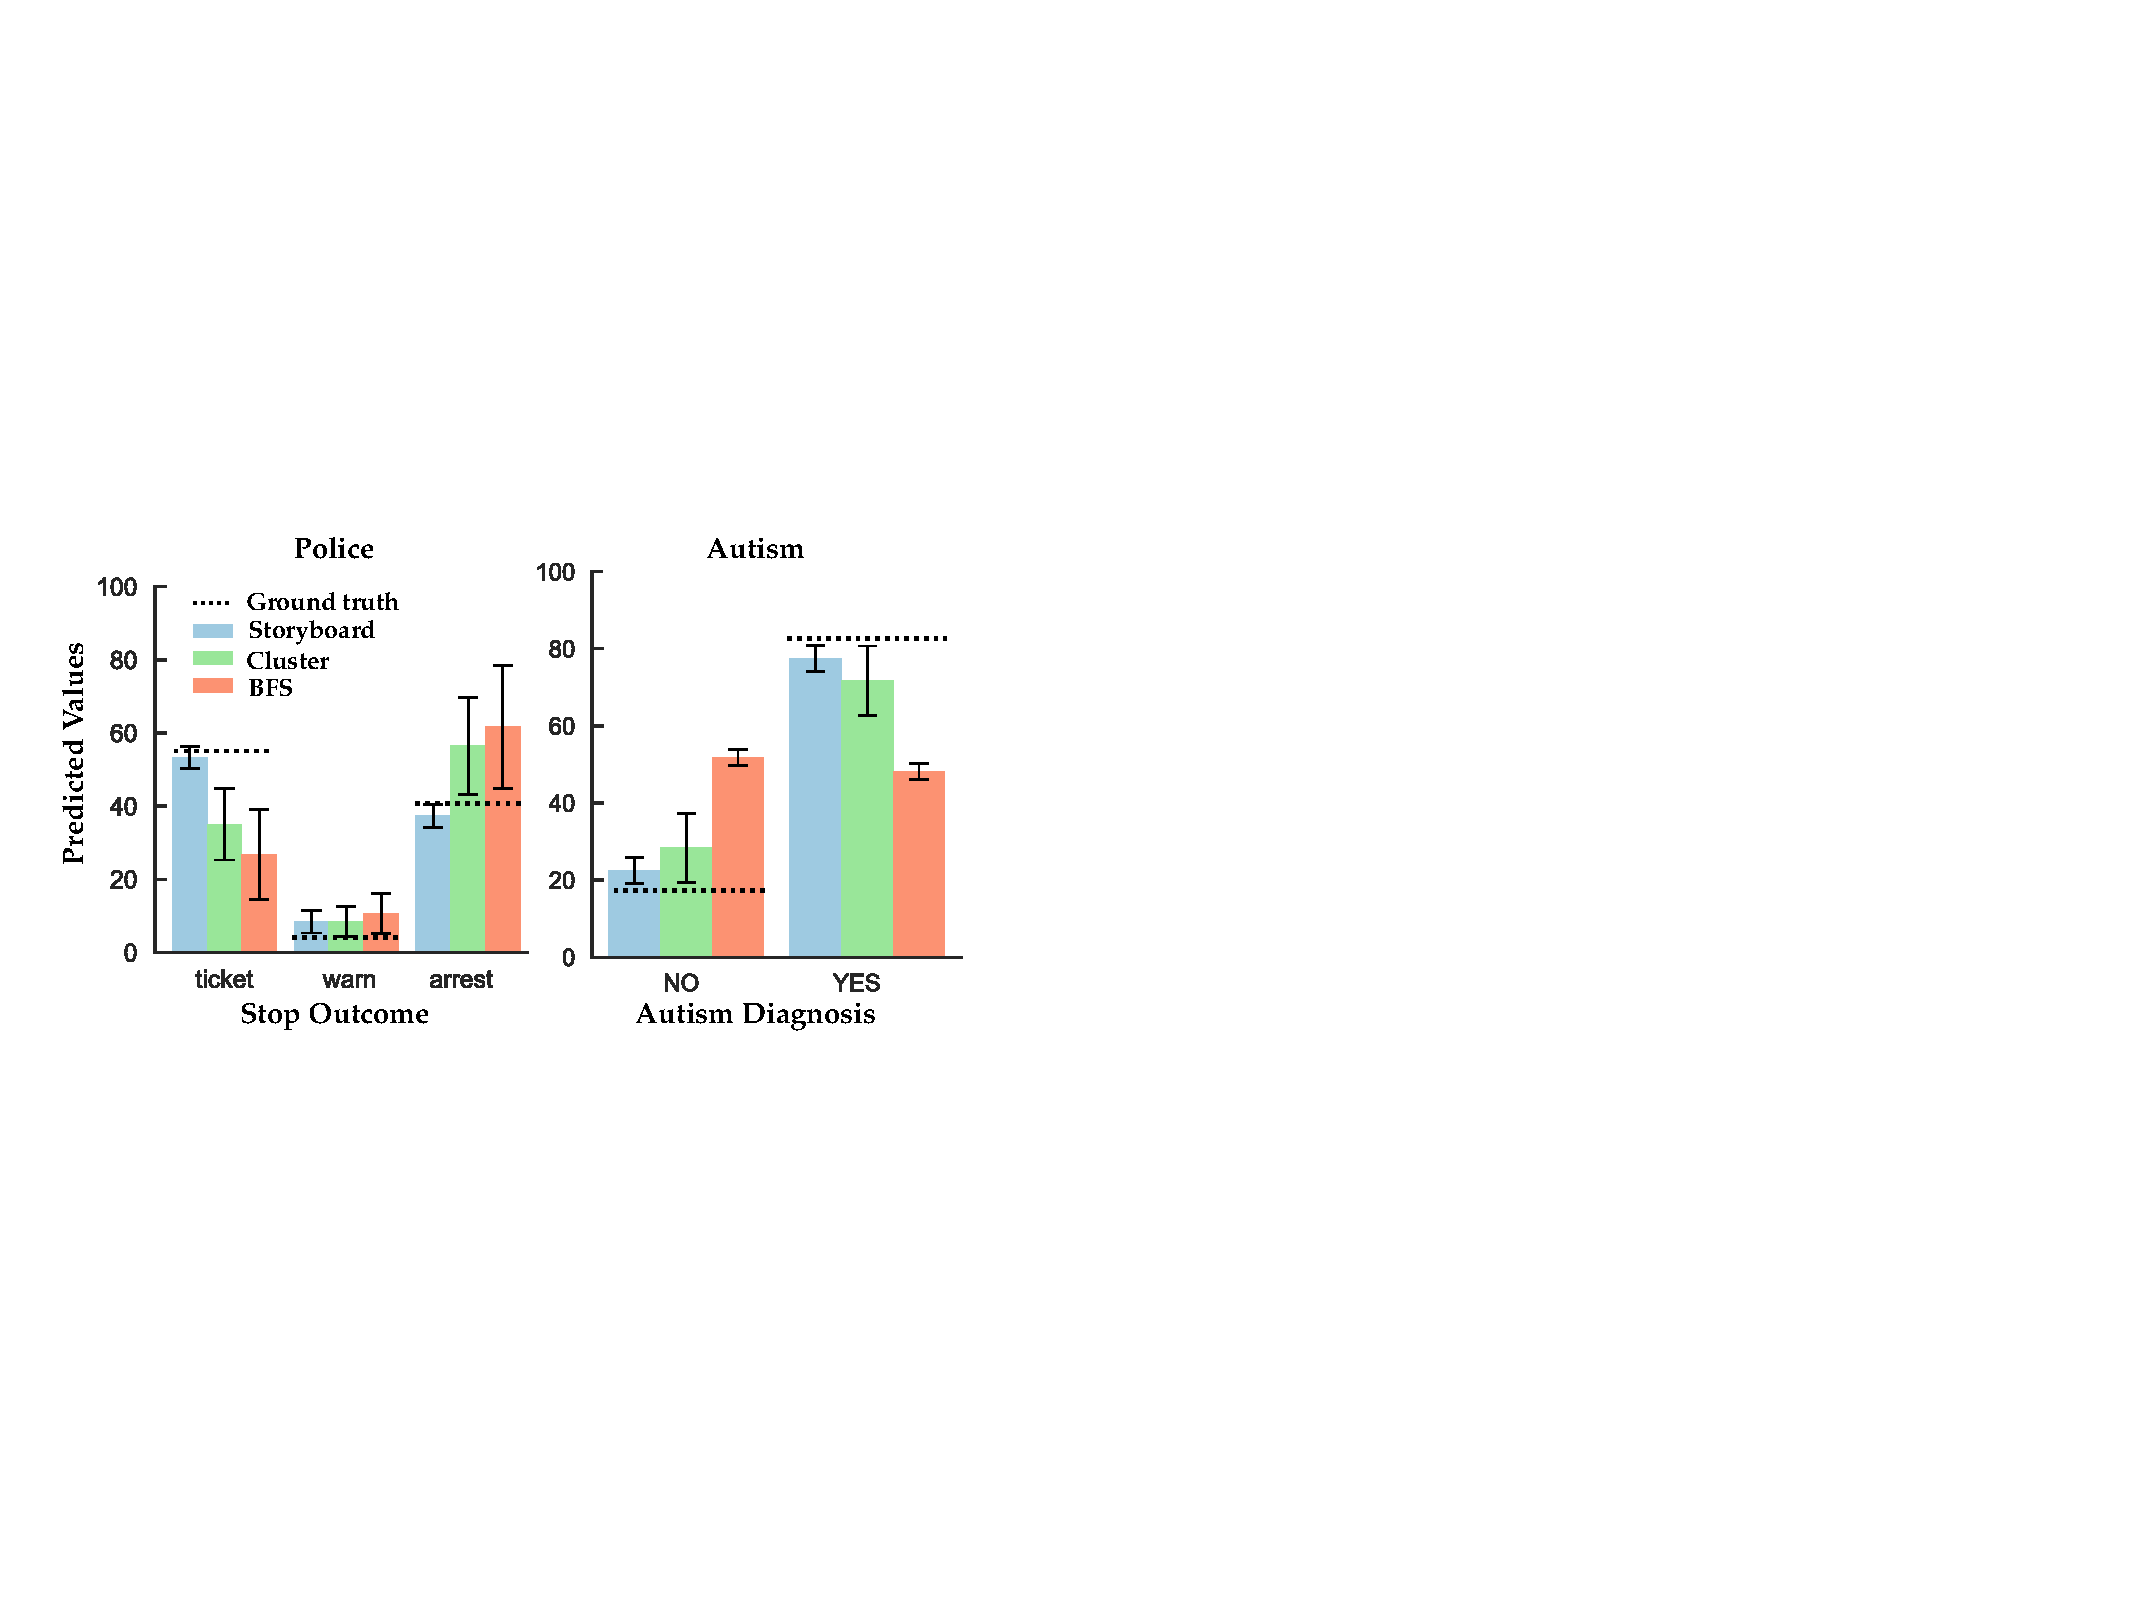
\includegraphics[width=0.85\linewidth]{figures/prediction.pdf}
\vspace{-10pt}
\caption{Mean and variance of predicted values. Predictions based on \system exhibit lower variance \change{(error bars)} and closer proximity to the ground truth values (dotted).}%\agp{Fix}
\label{fig:actual_predictions}
\vspace{-10pt}
\end{figure}
\change{
	\stitle{RQ3: How well does the dashboard convey information regarding \change{the} \emph{overall} dataset schema?}% information regarding the relative importance of different attributes
\npar
\change{We use the common  task
of judging the relative importance of attributes
as an indicator of the participants' overall understanding.}}
To determine \change{ground truth} attribute importance,
we computed the Cramer's V statistics
between attributes to be ranked
and the attributes of interest.
Cramer's V is \change{commonly used for}
determining
the strength of association between categorical attributes~\cite{McHugh2013}. We deem an attribute as important if it has one
of the top-three\footnote{\change{This relevancy cutoff is visually-determined via the elbow method to indicate which rank the Cramer's V score drops off significantly.}} Cramer's V scores amongst all attributes of the dataset.
For the list of rankings provided by each participant,
we first remove attributes \change{that} participants chose not to rank.
We compute the F-scores and average precision (AP) at k
\change{relative to the ground truth
for various values of $k$}
\tr{(from 1 up to the number of ranked attributes, with k values corresponding to attributes ranked as ties deduplicated)\agp{I don't understand this parenthetical note so I have moved it to the TR)}}.
Table \ref{table:ranking_results} \change{reports the average across participants} in each condition, after picking the best performing $k$ value for each \achange{participant} based on F-score and AP respectively. Both measures capture how accurately participants were able to \change{identify}
the three most important attributes for each dataset.
\begin{table}[ht!]
	\centering
	\vspace{-10pt}
	\begin{tabular}{lllll}
	         & \multicolumn{2}{c}{Police}                                   & \multicolumn{2}{c}{Autism}                                   \\ \hline
	Metric   & F                             & AP                            & F                             & AP                            \\ \hline
	\system  & \cellcolor{blue!25}0.750 & \cellcolor{blue!25}0.867 & 0.723                         & 0.600                         \\
	\cluster & 0.739                         & 0.691                         & \cellcolor{blue!25}0.725 & \cellcolor{blue!25}0.665 \\
	\BFS     & 0.739                         & 0.592                         & 0.222                         & 0.200                         \\
	\end{tabular}
	\caption{Best AP and F-scores for the attribute ranking task.}
	\label{table:ranking_results}
	\vspace{-20pt}
\end{table}
\par
\change{For this task,
we expected \BFS to have an inherent
advantage,
since \BFS dashboards consist of all univariate distributions,
providing more high-level\achange{, ``global''} information regarding each attribute.
However,}
both \system and \cluster (which contained more ``local'' information)
performed better than \BFS. The problem with \BFS is that given \change{a limited dashboard \achange{budget} of $k = 10$ visualizations that could be displayed, not all univariate distributions were shown}.% or real-estate
For the Police dataset, it happened to select several
important attributes (related to contraband and search)
to display in the first 10 visualizations.
However, \change{for Autism,}
only visualizations \change{corresponding to}
binary diagnostic
questions 1-4 fit in the dashboard.
So the poor ranking behavior comes from the fact that
the \BFS generated dashboard failed to display
the three most important attributes (questions 5, 6 and 9)
given the limited budget.
This \change{demonstrates \BFS's lack of
consistency across different datasets,
due to the fact that exhaustive exploration
can only lead to limited understanding of the data.}

\par We see that \system\ performs better
than \cluster for the Police dataset
and closely follows \cluster for the Autism dataset.
It is not entirely surprising that \cluster did well,
since it is a well-established method for
summarizing high-dimensional data~\cite{Han2005}.
For Autism, \cluster happened to pick the majority of visualizations (8/10) as univariate distributions that exhibited high-skew and diversity,
leading to more informed inference \change{of} attribute importance.
Since clustering seeks visualizations
that exhibit diversity in the shape of the data distributions,
it could potentially result in visualizations with many filter combinations.
For the police dataset, 6 out of 10 visualizations had
\change{more than 2} filters,
making it difficult to interpret \change{the visualization}
without \change{an} appropriate context to compare against.

\par \change{Overall,} both \BFS and \cluster
do not provide consistent guarantees for highlighting important visualizations across different datasets. In general, our results indicate that \change{participants} gain a better \change{\emph{overall} dataset} understanding regarding attribute importance using \system, with only a few \change{targeted visualizations that tell the ``entire story''. This is without \system being explicitly optimized
for the ranking task}.

%!TEX root = main.tex
\change{\section{Discussion of Study Results}}
To \bchange{further understand how participants 
made use of the recommended visualizations during their analysis}, 
we analyzed the user study \bchange{transcripts}
through an open coding process~\cite{Muller1993} by two of the authors. 
For each task in our study, we assigned a binary-valued code to indicate whether or not a participant engaged in a particular action or thought process. Table~\ref{table:thematic_summary} highlights results from thematic coding discussed in this section. We will use the notation [Participant.DatasetAlgorithm] to refer to a participant engaging with a dashboard created by an algorithm=\{1,2,3\}=\{\system, \cluster, \textsc{BFS}\} on a dataset =\{A,B\}=\{Police, Autism\}.
% \stitle{\system promotes distribution-awareness by provoking comparisons against more informative contextual references.}We first studied the thematic codes to understand how participants select contextual references for visualizations.
\subsection{The Choice of Contextual References}
\par As discussed earlier, 
analysts often make use of 
related visualizations to 
form their expectations for 
unseen \bchange{visualizations}. 
We refer to \bchange{the}
visualizations used 
for such purposes as \emph{contextual references}. 
\bchange{The appropriate choice
of a contextual reference (such as an informative parent)
is necessary to ensure the \emph{safety} of
insights derived through drill-downs.} 
To understand how ``safe'' the dashboards 
generated from each condition were, 
we examined \change{the visualizations} 
that participants compared against 
to form their expectations \change{for unseen visualizations}. 
In particular, we thematically encoded 
\bchange{the}
participants' use of contextual references 
based on \change{their} verbal explanations 
\change{for justifying} their prediction task responses. 
As shown in Table \ref{table:contextualReferenceCount}, 
in general, we find that participants make more comparisons in total using \system than compared to \cluster and \BFS.
\begin{table}[h!]
\vspace{-5pt}
\centering
	\begin{tabular}{l|rrrr|r}
	 \small{Algorithm}   &    \small{Parent} &   \small{Sibling} &   \small{Relative} & \small{Overall} &   \small{Total} \\
	\hline
	 \small{\system}     &    \cellcolor{blue!25} 12 &       8 &     0 &  11 &      \cellcolor{blue!25} 31 \\
	 \small{\cluster}     &         4 &        0 &         7 &          8 &      19 \\
	 \small{\BFS}         &         0 &        5 &         1 &          8 &      14 \\
	\end{tabular}
\caption{Out of 12 participants, the number of participants who made use of each contextual reference across the two datasets. Participant behavior shows a similar trend in individual datasets. \system participants made more comparisons in general and against parents compared to the baselines.}
\label{table:contextualReferenceCount}
\vspace{-20pt}
\end{table}
\par Participants can (and often do) make comparisons against more than one type of contextual references to obtain their prediction. We uncovered four main classes of contextual references, described below using the 
example visualization $V_i$=\texttt{\origcolor{gender=F, race=White, age=21-30}} (in the order of most to least similar to $V_i$) and illustrated in Figure~\ref{fig:reference}:
\begin{enumerate}
	\item \textbf{Parent} : Comparison against a visualization with one 
	filter removed (e.g., \texttt{\origcolor{gender=F, race=White}})
	\item \textbf{Siblings} : Comparison against a visualization that shares the same parent. In other words, the \bchange{filtered attributes are the same, but one filter has a different value}. (e.g., \texttt{\origcolor{gender=F, race=White, age=}\diffcolor{60+}})
	\item \textbf{Relatives} : Comparison against a visualization that shares some common ancestor (excluding overall), but not necessarily the same parent. \bchange{These} visualizations share at least one \bchange{common filter, but with more than one filter or filter value being different}\agp{I updated it based on what I thought this should have been--see figure for more}. (e.g., \texttt{\origcolor{gender=F, race=White, age=}\diffcolor{60+, search conducted=T}})
	\item \textbf{Overall} : Comparison against the distribution that describes the overall population (no filters applied).
\end{enumerate}
\begin{figure}[h!]
\centering
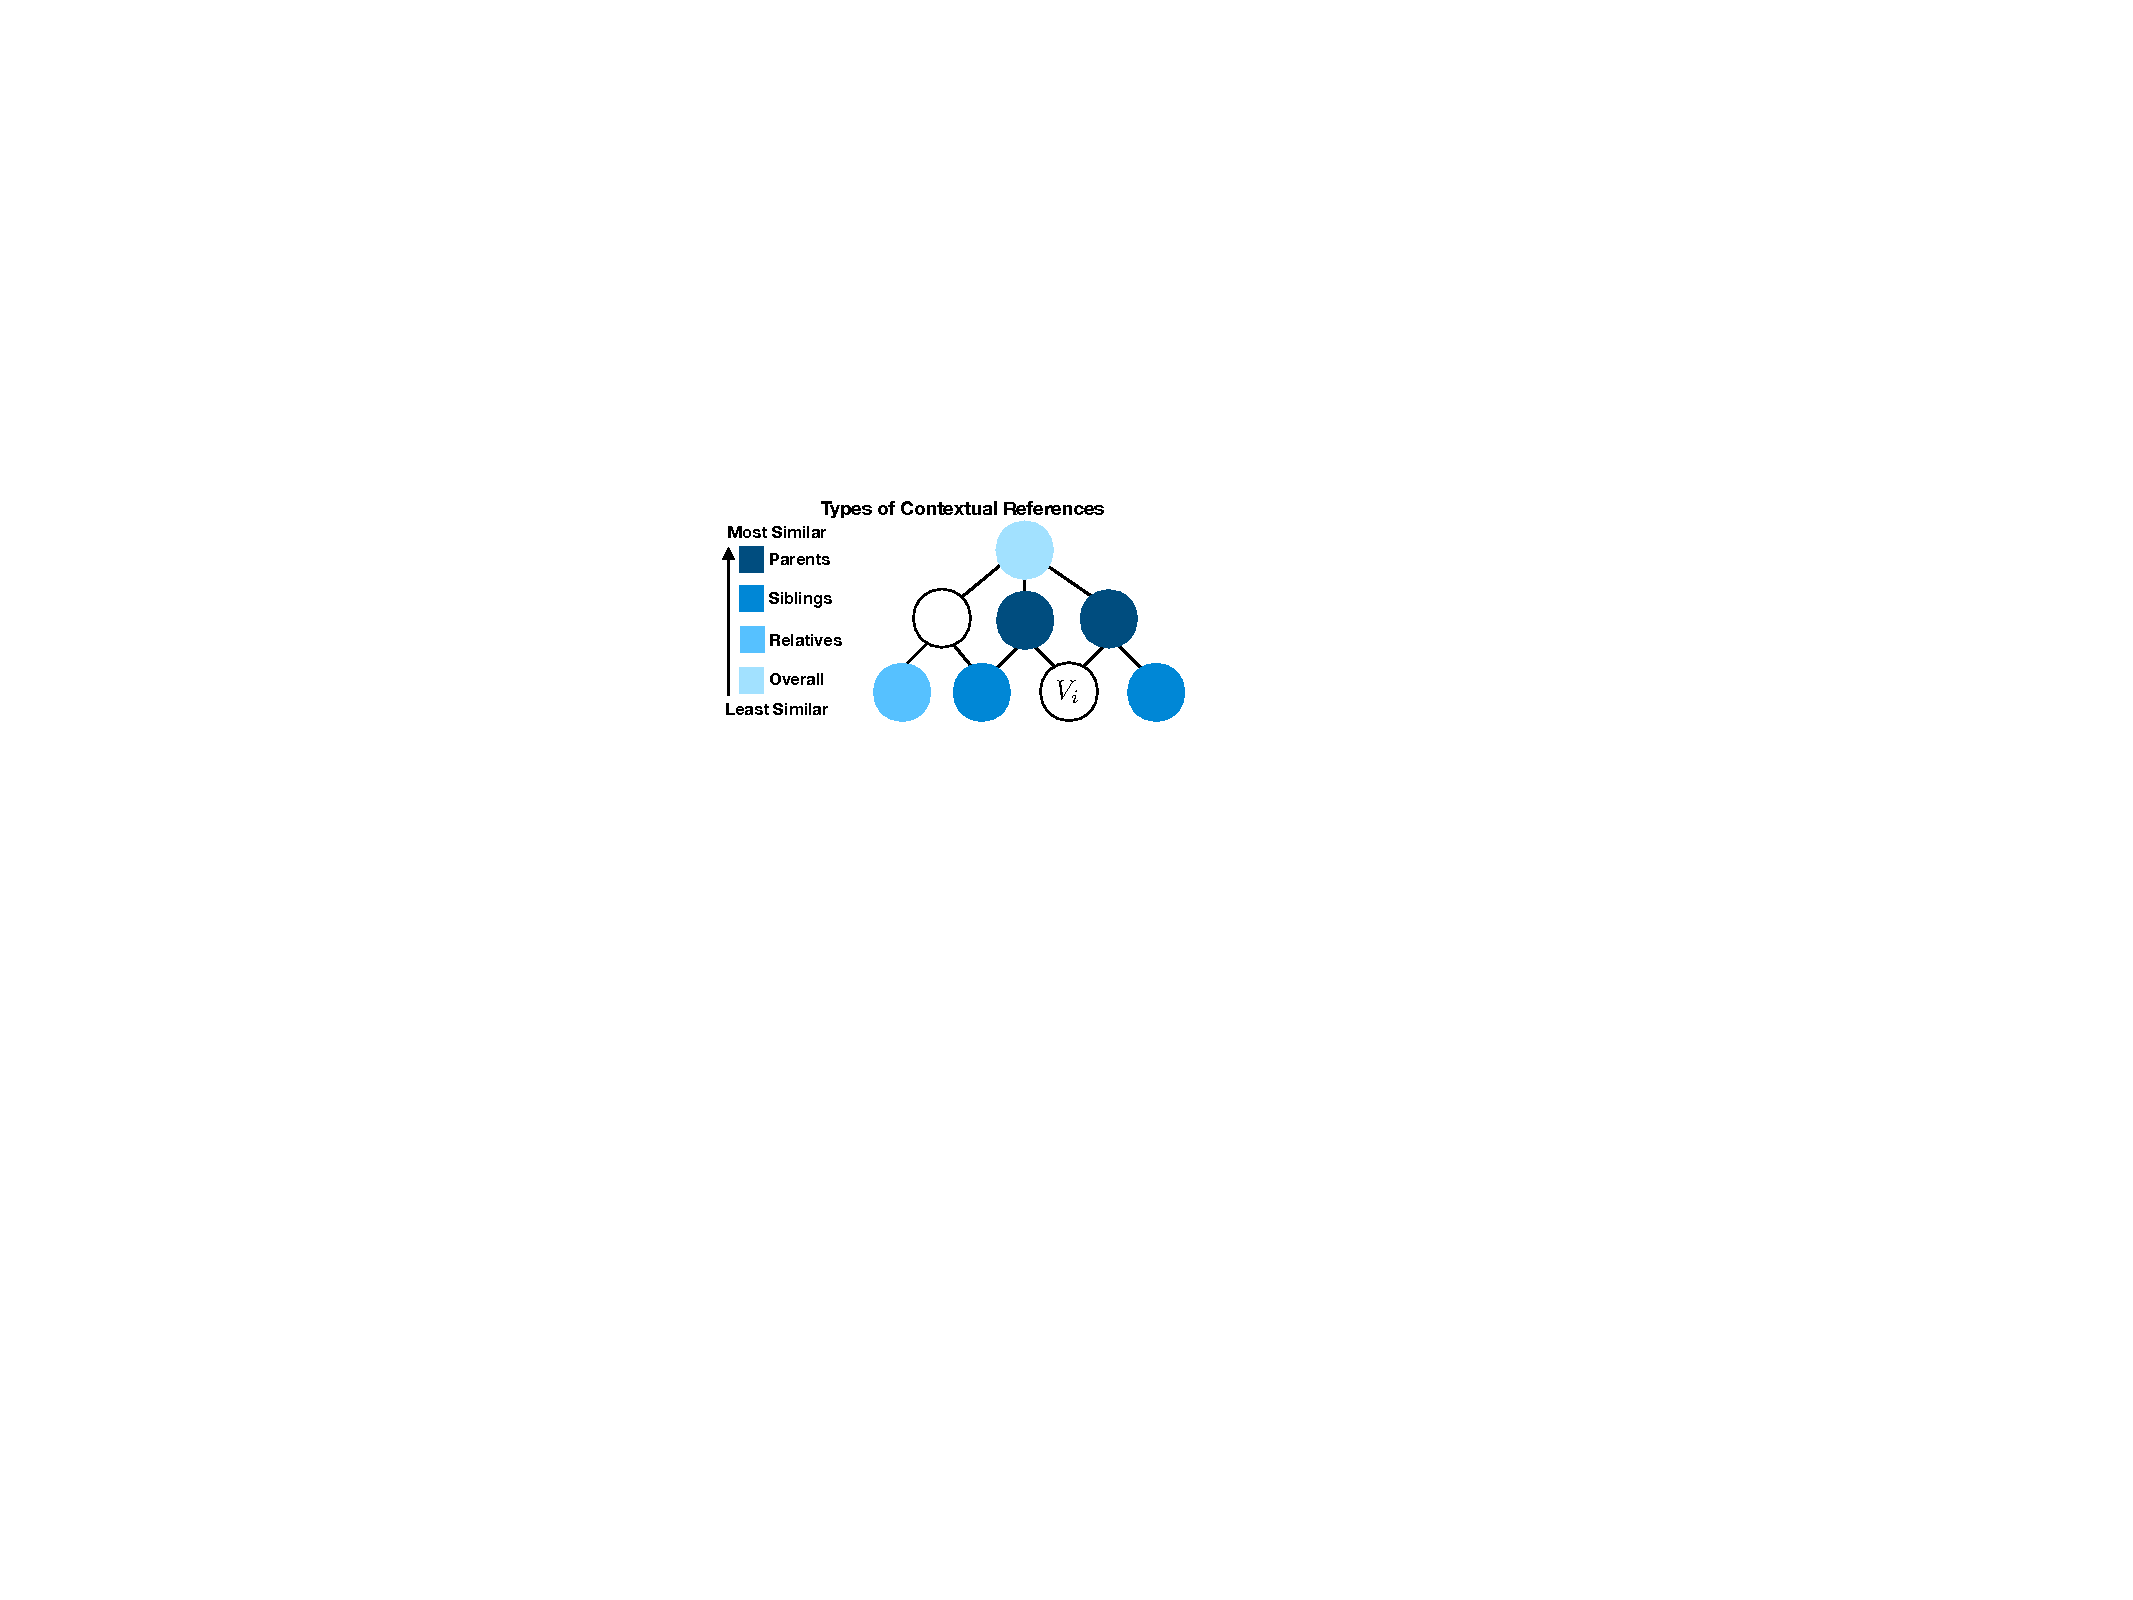
\includegraphics[width=0.7\linewidth]{figures/contextual_reference.pdf}
\caption{\change{Different types of contextual references} for a given visualization of interest $V_i$. The degree of similarity with respect to $V_i$ is denoted by darkest to lightest color hue.\agp{I don't see how the relative is actually a relative. It shares no similarity with $V_i$, and is no different from the other white node. (One way to see this is that the common ancestor for both the so-called relative and the white node and $V_i$ are the same -- the overall one.)}}
\label{fig:reference}
\vspace{-10pt}
\end{figure}
\par \change{Studying participants' use of contextual references reveals inherent challenges that arise from using the dashboards generated by \BFS and \cluster.} For \cluster, participants mainly compared against relatives and overall visualizations. Since \cluster optimizes the diversity of shape distributions amongst the visualizations, the selected visualizations had up to 4 filters and were disconnected from each other. For this reason, in many cases\change{,} participants could only rely on relatives and the overall visualizations as contextual references. For example, P4.A2 pointed at a 4-filter visualization with extreme values (100\% for warning; 0\% for arrest and ticket) and indicated how ``\textit{a lot of [the visualizations] are far too specific. This is not very helpful. You can't really hypothesize that all people are \change{[sic]} going to be warned, because it is such a specific category, it might just be one person}''. %, you need to have a bigger dataset. And that category will not really give you such extremes to make it more credible''.
He further explained how he ``\textit{would not want to see the intersections [(visualizations with many filters)] at first and would want to see all the bases [(univariate summaries)] then dig in from there.}'' The lack of informative contextual references in the \cluster dashboard is also reflected in how analysts exhibited high variance and deviation in their prediction responses. Note that the prediction task was chosen so that exactly one parent must be present in the dashboard, so these results do not point to the absence of parent visualizations in these \change{dashboards}, but rather indicate how participants made use of the information presented in the dashboards to form their prediction.
\par Furthermore, \change{improper comparisons against contextual references often make} it difficult for analysts to \change{interpret} displayed visualizations. In particular, when visualizations composed of multiple filter conditions were shown in \cluster dashboards, 25\% of participants had trouble \change{making sense of the meaning of a filter} for at least one of the datasets \change{(e.g., understanding that \texttt{gender=F AND age=60+} corresponds to female drivers with ages larger than 60 years old) at some point during the study}. In contrast, as shown in Table~\ref{table:thematic_summary}, this confusion only happened once for \BFS and none for \system. This is due to the fact that \cluster dashboards \change{seemed} random to the users, making it challenging to find ``close'' contextual references to compare against and form an accurate mental model. \change{In contrast, the linear ordering of \BFS and hierarchical ordering of \system were natural and interpretable for participants}. %In contrast, \BFS follows a linear ordering and \system follows a hierarchical ordering, which were more natural and interpretable for participants.
%despite our modification to KMeans which picks the visualizations with the least number of filters to show in the dashboard for improving interpretability
%These themes are drawn from user's explanations of how they obtained certain insights or ---- that --different tasks or while interpreting the dashboards. 4 categories :
\par For \BFS, most comparisons were based on the overall and siblings. Due to the sequential level-wise picking approach, the overall visualization for \BFS dashboards corresponded to the immediate parent, so they are not explicitly recorded as a parent. While the overall and sibling comparisons can be informative, \change{the incomplete comparisons, due to the limited number of first-level visualizations displayed, can result in flawed reasoning, likewise observed in the aforementioned Autism prediction task.} In contrast, for \system, almost all users compared against the overall and parents, while some also exploited \change{sibling comparisons} to make weaker guesses for less-frequently observed attributes (e.g., using a 2-filter sibling visualization involving \texttt{driver\_age} to infer another 2-filter visualization involving \texttt{driver\_age} with a different parent.)
% \subsection{Improper contextual reference can lead to misleading insights.}
\begin{table*}[ht!]
	\centering
	\begin{tabular}{|l|l|l|l|}
	\hline & \system & \cluster & \BFS \\ \hline
	Difficulty with Interpreting Visualizations & 0 & \cellcolor[HTML]{FD6864}3 & 1 \\ \hline
	Misjudged Significance of Potential Small-Size Population & 0 & \cellcolor[HTML]{FD6864}4 & 1 \\ \hline
	Interpretable ``Human-like" Dashboard & \cellcolor[HTML]{9AFF99}5 & 1 & 0 \\ \hline
	Number of Insights (Police) & \cellcolor[HTML]{9AFF99}11 & 8 & 9 \\ \hline
	Number of Insights (Autism) & \cellcolor[HTML]{9AFF99}16 & 6 & 11 \\\hline
	\end{tabular}
\caption{Summary of qualitative insights from thematic coding. We record the total number of insights based on overall \change{dataset findings} that \change{were} independently discovered by more than two different participants. For each participant, we coded the absence or presence of 7 such insights for the Police dataset and 6 insights for the Autism dataset.}%findings regarding the dataset or information regarding one or more attributes
\label{table:thematic_summary}
\vspace{-15pt}
\end{table*}
% \subsection{The Danger of Improper References}%, echoing our previous concern regarding the danger of small subpopulation sizes. This issue stems from the fact that the contextual reference used for comparison was the overall population, however the unseen parent subpopulation may have behaved very differently.
\tr{
	\subsection{The Danger of Small Subpopulations}
	The danger of spurious patterns and correlations in visualizations that contain small subpopulation size is a well-known problem in exploratory analysis~\cite{Binnig2017}. When examining visualizations with many filters and extremely-skewed values in one or more bars (bars with 100\% or 0\%), 4 \cluster participants did not realize that charts with multiple filters may have a smaller subpopulation size. In contrast, 6 of the participants using \system explicitly noted that while these extreme-valued visualizations may be interesting, they were less certain due to the unknown subpopulation size and should be investigated further. For example, P1.A1 noted that a visualization with warning=100\% caught her eye, ``\textit{but I don't know what the N is, maybe it's one person, this makes me a little skeptical, that makes me want to go back to the raw data and look at what is the N and what drives something so drastic?}'' We also found that this subpopulation-size fallacy was observed to be more severe for the Autism dataset, where participants had less intuition on the expected attribute behavior.  Since \BFS dashboards only displayed first-level visualizations, participants for \BFS did not see visualizations with large numbers of filters that had small subpopulations during the study, so none of the \BFS participants exhibited signs of this fallacy.
}
% \subsection{Hierarchical layout leads to more natural contextual comparisons compared to table layout.}
%it was easier to follow contextual references in \system
\subsection{Interpretability of Hierarchical Layouts}
\par In the post-study interviews, participants cited hierarchical layout as \change{a} key reason \change{for why they preferred \system recommendations}. \change{Even though participants were never explicitly told what the edge connections between the visualizations meant during the study, they were able to interpret the meaning of the dashboards effortlessly through \system's hierarchical layout}. For example, P1.A1 stated that ``\textit{the hierarchical nature [is] a very natural flow...so when you are comparing, you don't have to be making those comparisons in your head, visually that is very pleasing and easy to follow.}'' %Likewise, [P8.A1] also stated that ``I like the different levels, it makes it very visually easy to figure out what you want to look at, if you want to look at the overall data, it's right there at the top for you, if you want to get more specific, you just follow a branch downwards, which I think is very intuitive.''
Likewise, P9 described how \system's hierarchical layout for the Autism dataset was a lot easier to follow than the Police dataset shown in the table layout for \cluster:
\begin{quote}
\textit{If I had to look at this dataset in the format of the other one, this would be much more difficult. It was pretty hard for me to tell in the other one how to organize the tree, if there was even a tree to be organized. I like this layout much better, I think this layout allows me to approach it in a more meaningful way. I can decide, what do I think matters more: the overall trend? or the super detailed trends? and I know where to look to start, in the other one, every time I go back to it, I would say, where's the top level, where's the second level? I mentally did this. Like when you asked me that first question, it took much longer to find it, because I literally have to put every chart in a space in my head and that took a lot longer than knowing how to look at it.}
\end{quote}
At the end of the study, some participants \change{who were assigned dashboard conditions with table layouts} sketched and explained how they would like the layout of the visualizations to be done. \change{These} participants expressed that they wanted ``groupings'' or layouts that arranged visualizations with the same attribute together. Other participants advocated for isolating the overall visualization outside of the dashboard table for facilitating easier comparisons. Both of these suggestions provide further motivation for our hierarchical organization of visualizations. \change{\papertext{Our findings echo prior work on visualization sequences and storytelling~\cite{Hullman2017,Segel2010,Boy2015,Kim2017}, which found that analysts prefer visualization sequences structured hierarchically based on shared data properties such as levels of aggregation ordered by increasing levels of summarization.}}
%Kim et al.~\cite{Kim2017} modeled relationships between charts by empirically estimating transition (edge) cost between moving from one visualization (node) to another. They found that participants preferred ``\textit{starting from the entire data and introducing increasing levels of summarization}''.
 %layout and the idea of the collapsed visualizations as described earlier.%in Section \ref{sec:interaction}.
\par Since we did not inform participants about how the dashboards were generated, it was \change{surprising to see} that some participants \change{presumed} that the dashboards were hand-picked by a human analyst and \change{hypothesized} what this \change{fictitious analyst}'s intentions were (e.g., ``\textit{It seems like the researcher who created this dashboard was specifically looking at people of Asian descent and people who are 60 or older.}'' [P7.A1]). \change{Table~\ref{table:thematic_summary} shows how} 5 out of 12 participants referred to the \system dashboards as if they were generated by a human, whereas there was only 1 participant for \cluster and none for \BFS made such remarks\change{\footnote{We encoded this phenomenon by looking at instances where a participant either explicitly \change{referred} to a person who picked out the dashboard or implicitly described their intentions through personal pronouns.}}. At the end of the study, many were surprised to learn that the \system dashboard was actually picked out by an algorithm, indicating that \system could automatically \change{generate convincing dashboards similar to ones that were} authored with human intention. The interpretability of \system dashboards may have contributed to the increased number of insights discovered in both datasets compared to the two baselines, as summarized in Table~\ref{table:thematic_summary}.
\stitle{Limitations of \system}
% Interestingness task is highly subjective, so not conclusive whether interesting or not , despite the positive result
% Due to the highly subjective nature of the retrieval task, the interestingness selection for the Police dataset was biased by participant's priors and intuition about the attributes. For example, while all participants who have seen the visualization "duration=30+min" verbally noted that stop duration is a crucial factor that leads to arrest, only 4 users marked it as interesting. 5 participants marked the visualization as not interesting and 4 left it unselected, because the visualization was not very surprising as it agreed with their intuition that ``\textit{if the police stop is taking a long time, something has probably gone wrong}''.
\par As described earlier, since the details of how the dashboards were obtained \change{were} not explained to the users during the study, some users expressed that they were initially confused by \system \change{as} not all variables were present in the dashboard. Others also found it confusing that the addition of filters did not always correspond to the same variables. For example, P2.A1 criticized how the dashboard was intentionally selected to be biased:
\begin{quote}
\textit{I feel like this one, not all the data is here, so we are already telling a story, you are trying to steer the viewer to look at certain things. And the focus seems to be on where the arrest rate is high. You probably could have found other things that led to ticket being high, but you didn't pull those out. You are trying to see if there are other factors that lead to more arrests.}
\end{quote}
\npar This sentiment is related to participants' desire to perform their own ad-hoc querying alongside the dashboard to inspect other related visualizations for verifying their hypothesis. For example, P7.A1 wanted to inspect all other first-level visualizations for driver's race to assess its influence. P7.A1 expressed that while he had learned many insights from the dashboard, ``\textit{the only thing I don't like is I cannot control the types of filter, which is fixed.}'' \change{Since the design objective for \system is to support and evaluate its capability to provide informative dashboards, \system is limited in its interactivity and the extent of free-formed data exploration it supports. This result also points to how} \system could serve as a helpful \change{assistant} alongside other conventional visualization tools, such as Tableau. Outside the context of the user study, it is essential to explain how \system \change{selects} the visualizations in \change{an} easy and interpretable manner to establish a sense of summarization guarantee for the users and help them make better inferences with the dashboard.

\change{%a small set of analytic tasks corresponding to each design objectives, with
	\par Since the goal of our study is to evaluate whether \system can assist users in drill-down exploration, our preliminary study is limited to comparison against baselines stemming from conventional approaches for multidimensional data exploration. While we understand how the \system study condition may confound both the hierarchical layout with the algorithmic choice of visualizations, our intention for the baseline was to simulate how analysts generate a large number of visualizations individually, typically arranged in a table grid layout, rather than using a hierarchical layout. Further evaluation comparing how the different hierarchically-displayed visualization selection algorithms assist users in drill-down exploration is a direction of future work.
}
\tr{
	\par As discussed earlier, subpopulation size is important in establishing the significance of a trend observed in a visualization. While subpopulation size is taken into account implicitly in our objective, we should design interfaces that convey the notion of subpopulation size in our dashboard. Examples include Sankey-like flow diagrams indicating the percentage of the parent population broken down into individual subpopulations and subpopulation size explicitly specified via edge labels.
}


%, either explicitly displayed as text when hovering over the visualization or changing the size or background color of the visualizations to encode subpopulation size.
%“I actually found it really confused at first because such a low arrest rate at the top, and then at the bottom the arrest rate was much higher, so I was like is this data wrong. Then I realized we’re not looking at all the data here, you’ve pulled out some of it. It took me a minute to realize that. And once I read the title of the charts I realized that makes sense.” [P2.A1]
% - Reference of Comparison
% - Layout naturally lends itself for comparison:
% 	- describe ordering layout, how participants naturally follow the flow
% 	- emph that we did not tell them what the edge connections mean and how they were computed but the users naturally figured it out, that it means adding an additional filter.
% 	- hierarchical interpretable nature (quotes)
% 	- compared to other baselines
% 	- describe dashboard by human (count)
% - Misleading insights v.s. True insight discovery rates
% 	- Interpretability:
% 	- misled understanding subpopulation size
% 		- for autism, it is important to see if they compare to overall because if not they would think high skew to NO is important whereas its actually pretty close to overall.
% 	- trouble interpreting filter combination
%%%%%%%%%%%%%%%%%%%%%%%%%%%%%%%%%%%%%%%%%%%%%%%%%%%%%%%%%%%%%%%%%%%%%%%%%%%%%%%%%%%%%%%%%%%%%%%%%%%%%%%%%%%%%%%%%%%%%%%%
%%%%%%%%%%%%%%%%%%%%%%%%%%%%%%%%%%%%%%%%%%%%%%%%%%%%%%%%%%%%%%%%%%%%%%%%%%%%%%%%%%%%%%%%%%%%%%%%%%%%%%%%%%%%%%%%%%%%%%%%
%%%%%%%%%%%%%%%%%%%%%%%%%%%%%%%%%%%%%%%%%%%%%%%%%%%%%%%%%%%%%%%%%%%%%%%%%%%%%%%%%%%%%%%%%%%%%%%%%%%%%%%%%%%%%%%%%%%%%%%%
% \subsection{Statistical Paradoxes}\dor{make title full sentences}
% Visualizations are powerful representations for studying different distributions or patterns in a dataset, but our human intuition could often mislead us when it comes to interpreting those patterns\cite{Binnig2017,Wall2017}. Several statistical paradoxes can lead analysts to draw incorrect conclusions from observed visualizations, including Simpson's paradox as discussed in the introduction. The key reason why many of these paradoxes emerge is the \emph{incompleteness} of the observed data or lack of focus on relevant informative subsets of the data. For example, Simpson's paradox arises in the presence of an unseen confounding variable. %likewise, the absence of  base rate information causes base rate fallacy.
%  We assert \dor{too strong of a sentence} that distributional awareness can be useful in avoiding such statistical paradoxes. If an analyst is aware of all distributions in a given dataset, he/she is less prone to many statistical paradoxes. However, given the large number of dimensions and high cardinality of these dimension in modern datasets, it is not possible for an analyst to explore and memorize all distributions. Therefore, a more evolved approach is to be aware of the exceptional distributions. In this work, we propose a first step towards this goal, where we identify the exceptional distributions in terms of their informative references. The remaining (unseen) distributions in the dataset are rather unsurprising and can be inferred from the visualizations in the dashboard. \dor{I would recommend first talk about issue with large dimension + danger of multiple hypothesis testing + incomplete testing, point out problem, then talk about how our system resolves this.}
% \subsection{Structural Insight}
% Our proposed dashboard consists of a hierarchy of visualizations, where each visualization is linked to its most informative parent. The shape or structure of the hierarchy contains useful information that augments the information learned from the visualizations and aid distribution awareness and understanding. \dor{what's interesting here is that while many work have looked at visualization presentation, layout of presentation never considered, we find in Sec 5 that this is actually important and can encode info.} For example, the depth and branching factor of the hierarchy could inform a user regarding the configuration of insights. Deep hierarchies contain long paths, i.e., insights are present at lower level visualizations with multiple constraints. In contrast, bushy hierarchies (with high branching factor) contain cases where multiple visualizations have the same informative parent and they differ from that parent. \dor{do we have examples from the study that support this?} We assert that the depth and branching factor could be a meaningful constraint in our problem formulation \dor{too strong of a sentence}. Some applications for example, funnel exploration require studying deep hierarchies, whereas others for example, building decision trees require studying bushy hierarchies. A natural extension of our current problem formulation is to allow users to select the depth and branching factor for the hierarchy.
% \subsection{Other Visualization Lattices}
% In this work, we explore the space of data subsets to generate our visualization lattice. Note that it is possible to explore the space of dimension attributes in x-axis to generate a different visualization lattice. In particular, given a combination of dimension attributes $X = \{X_1, \ldots, X_n\}$, adding one or more new dimensions in $X$ will generate a new combination. An ancestor-descendant relationship exists between these dimension combinations, following the same principles of Section 3.1. These relationships lead to a new lattice, which we call the dimension combination lattice. Our informative deviation based approach could be used for traversing the dimension combination lattice. However, we observe that most users do not visualize more than two attributes in x-axis. Therefore, traversing the dimension combination lattice is not very useful for most applications.
% \dor{I think 6.2,6.3 don't tie well with the rest of the paper. It sounds like stretching our own ideas rather than being motivated by the work done in this paper. Other potentially more relevant discussion: distribution awareness and how it might be useful in other contexts? Decision trees?}
% %\subsection{Utility Metrics}

%!TEX root = main.tex
\section{Other Related Work\label{sec:related}}
Our work draws from past research in multidimensional data exploration and fallacies in visual analytics\change{; we discuss work that we haven't covered so far in this section}. %\agp{Can we edit this so that it's not repeating what is in S1?} %\change{Other less-relevant past work on decision tree visualization and visualization storytelling is included as reference in the technical report.}
\stitle{Guided Exploration of Multidimensional Data.}
Given a dataset, tools such as Tableau support automatic generation of visualizations based on graphical presentation rules~\cite{Mackinlay2007,Wongsuphasawat2016}.
A more recent body of work automatically selects visualizations based on statistical measures, such as scagnostics and deviation. \achange{For discovering interesting conditional structures in scatterplots}, Anand et al. \cite{Anand2015} \change{apply} randomized permutation tests to select partitioning variables that \change{reveal} interesting small multiples using scagnostics\change{~\cite{Dang2014,Wilkinson2005}}. \bchange{For recommending visualizations for assessing data quality, Kandel et al.~\cite{Kandel2012} uses mutual-information as a distance metric for recommending views that highlight anomalies, as well as related views that explains the value distribution of the anomalous views. 
Vartak et al.~\cite{Vartak2015,DBLP:journals/pvldb/VartakMPP14} uses deviation
to recommend visualization attributes that highlight differences in two populations,
while Siddiqui et al.~\cite{Siddiqui2017} and Macke et al.~\cite{Macke2018} employ
deviation to find similar visualizations. 
Qetch~\cite{Mannino2018QetchTS} and ShapeSearch~\cite{DBLP:journals/corr/abs-1811-07977} craft more sophisticated deviation measures to identify visualizations of interest.} Our work extends \achange{these} deviation-based \bchange{measures} to formulate user expectation. However, unlike existing \bchange{work}, we concentrate on informativeness \achange{rather than the exhaustive enumeration of the entire space}, which enables our system to avoid drill-down fallacies. %Given a bar chart, Vartak et al. \cite{Vartak2015} \change{find} other interesting bar charts that deviate from the input chart using a deviation-based measure.
%\cite{Elmqvist2008Rolling} presents an interactive tool to explore multidimensional data using a matrix of scatterplots that shows the relationship between all pairs of attributes.
% \dor{add smart drill-down~\cite{Joglekar2015}}
\stitle{Preventing Biases and Statistical Fallacies.}
Visualizations are powerful representations for discovering trends and patterns in a dataset; however, cognitive biases and statistical fallacies could mislead analysts' interpretation of those patterns~\cite{Alipourfard2018WSDM,Wall2017,Zgraggen2018CHI,Armstrong2014,Gotz2016}. Wall et al.~\cite{Wall2017} \change{present} six metrics to systematically detect and quantify bias from user interactions in visual analytics. These metrics are based on coverage and distribution, which focus on the assessment of the process by which users sample the data space. Alipourfard et al.~\cite{Alipourfard2018WSDM} presents a statistical method to automatically identify Simpson's \bchange{paradoxes} by comparing statistical trends in the aggregate data to those in the disaggregated subgroups. Zgraggen et al.~\cite{Zgraggen2018CHI} \change{present} a method to detect the presence of the multiple comparisons problem in visual analysis. \bchange{This paper, on the other hand, focuses} on a novel type of fallacy \bchange{that occurs} during drill-down exploration that has not been addressed by past work. %drill-down fallacy, a fallacy that has not been addressed before in visual analytics literature.
\tr{
  \subsection{Decision Tree Visualization}
  The popularity of decision trees in a variety of classification tasks have led to the development of visualizations that make these models more interpretable~\cite{Ankerst1999,Hermann2017,Terence2018}. These visualizations often contain a visual representation of the rules as paths connecting the decision nodes, illustrating the proportion of sample along different paths, as well as statistics regarding the prediction accuracy at every node. Though our dashboards visually look similar to decision trees, the underlying objectives are different for the two methods. During tree construction, a decision tree algorithm aims to improve the classification accuracy of a target variable, typically by minimizing the entropy of distribution from parent node to child node~\cite{Quinlan1986}. In contrast, our method aims to deliver informative insights, by maximizing the informative deviation between parent and child nodes. Consequently, the generated outcomes are different for the two methods---a decision tree well explains the general rules (e.g., if stop duration is more than 30 minutes, the driver has 60\% probability of being arrested), whereas our method well explains the exceptions (e.g., if a stop duration is more than 30 minutes and the driver's race is Asian, the probability of arrest goes down to 35\%). Note that the general rule is useful for predicting the stop outcome for an unlabeled test datapoint (classification), whereas the exception is useful for realizing when the general rule no longer holds (insight). The latter insight may not be discovered by a decision tree as it does not directly improve classification accuracy. Another key difference between the two methods is \emph{coverage}---a decision tree covers the entire dataset (consistent with its classification goal), whereas our method highlights only the interesting regions of a dataset (consistent with its insight goal).
  \subsection{Storytelling with Visualization Sequences}
  Visualizations are often arranged in a sequence to narrate a data-driven story. Existing work on visualization sequences and storytelling has studied the structures of narrative visualizations~\cite{Hullman2017,Segel2010}, effects of augmenting exploratory information visualizations with narration~\cite{Boy2015} and, more recently, ways to automate the creation of visualization sequences~\cite{Hullman2013,Kim2017}. Most of these work have adopted a linear layout (motivated by slidedecks) to present the visualization sequences. Hullman et al.~\cite{Hullman2017} found that most people prefer visualization sequences structured hierarchically based on shared data properties such as levels of aggregation. Kim et al.~\cite{Kim2017} modeled relationships between charts by empirically estimating transition (edge) cost between moving from one visualization (node) to another. They found that participants preferred ``\textit{starting from the entire data and introducing increasing levels of summarization}''. Our work is the first to automatically organize visualizations in a hierarchical layout for summarizing data distributions across the space of data subsets.
}

%!TEX root = main.tex
\section{Conclusion}
\par Common analytics tasks, such as causal inference, feature selection, and outlier detection require studying data distributions at different levels of data granularity~\cite{Anand2015,Heer2012,Wu2013,Hullman2017}. However, without knowing \textit{what} subset of data contains an insightful distribution, manually exploring distributions from all possible data subsets can be tedious and inefficient. Moreover, when examining data subsets by adding one filter at a time, analysts can fall prey to the drill-down fallacy, where they mistakenly attribute the interestingness of a visualization to a ``local difference'', while overlooking a more general explanation for the root cause of the behavior. To address these issues, we presented \system, an interactive visualization recommendation system that automatically selects a small set of informative and interesting visualizations to summarize key distributions within a dataset. Our user study demonstrates that \system can guide analysts towards more informed decisions for retrieving interesting visualizations, judging the relative importance of attributes, and predicting unseen visualizations, than compared to two \change{other baselines}. Study participants also find dashboard generated by \system to be more interpretable and ``human-like'', leading to more discovered insights. Our work is one of the first automated systems that guides analysts across the space of data subsets by summarizing key insights with safety guarantees---a step towards our grander vision of developing intelligent tools for accelerating and assisting with visual data discovery.  
% discovery
% - Drill down is hard and dangerous
% - Drill down fallacy
% - In this paper, we develop ----
% - \system does X, Y , Z
% Our user study shows that ----\system compared to baselines
% 	- perform better in a wide range of analytic task such as attribute ranking, prediction, and interestingness.
% 	- interpretable, more insights
% - Wider implications

\newpage
\bibliographystyle{SIGCHI-Reference-Format}
% \bibliographystyle{ACM-Reference-Format}
\bibliography{reference}

\end{document}
